\chapter{Sums of random variables}

\section{Convergence: Law of Large Numbers}
\label{sec: law of large numbers}

The difference between a ``weak law'' and ``strong law'' is the convergence type.
A ``weak law'' only requires convergence in probability, while a ``strong law''
requires almost sure convergence. The typical strategy to obtain strong laws is
to obtain quantitative convergence results in expectation (e.g. in \(L^p\)), translate them
to quantitative convergence result in probability using the Markov inequality
and deduce almost sure convergence using the Borel-Cantelli lemmas from
the rate of convergence, that is
\[\begin{aligned}
    \substack{\text{Qunatitative}\\ X_n \overset{L^p}\to X } \quad
    \overset{\text{Markov ineq.}}\implies \quad \substack{\text{Quantitative}\\ X_n \overset{p}\to X}\quad
    \overset{\text{Borel-Cantelli}}\implies \quad X_n \overset{\as}\to X.
\end{aligned}
\]
The reason for this strategy is that it is often easiest to calculate
expectations.  For example \(\norm{X - \E[X]}_{L^2} = \sqrt{\var{X}}\). 
In this section we illustrate this strategy by implementing it for the
law of large numbers. It turns out that the natural domain to work in
is a Hilbert space \((\hilbert, \inner{\cdot, \cdot})\) as it allows
the definition of the covariance and variance in a natural way.

\begin{remark}[Expectation in multiple dimensions]
    \label{rem: expectation in multiple dimensions}
    In the discrete case, the expectation is
    \[
        \Exp{X} = \sum_{x} x \Prob{X = x}
    \]
    Observe the key for this to work is that the \(x\) are summable and scalable
    by a scalar probability. This only requires a vector space structure.  
    In general the expectation is defined via integrals -- specifically the
    ``Bochner integral'' in infinite dimension. We will not go into the measure
    theoretical details here. Simply understand that the expectation is a linear
    and therefore an ``entrywise'' operation acting on the basis due to
    \[
        \Exp{X}
        = \Exp[\Big]{\begin{pmatrix}
            X^{(1)} \\
            \vdots \\
            X^{(\dims)}
        \end{pmatrix}}
        = \Exp[\Big]{\sum_{i=1}^\dims X^{(i)} e_i}
        \overset{\text{linear}}= \sum_{i=1}^\dims \Exp{X^{(i)}} e_i
        = \begin{pmatrix}
            \Exp{X^{(1)}} \\
            \vdots \\
            \Exp{X^{(\dims)}}
        \end{pmatrix}.
    \]
\end{remark}

\begin{definition}[Covariance]
    \label{def: covariance and variance definition}
    Let \(X, Y \in \cL^2(\hilbert)\), then their \textbf{covariance}
    and \textbf{variance} are defined as
    \[
        \cov{X}{Y} \coloneq \Exp[\Big]{\inner[\big]{X-\Exp{X}, Y-\Exp{Y}}}
        \quad \text{and} \quad
        \var{X} \coloneq \cov{X}{X}.
    \]
\end{definition}

\begin{remark}
Note that \(\covSymb\) is an inner product and we will later define
a covariance operator \(\CovSymb\) that is an outer product such that \(\covSymb\)
becomes the trace of \(\CovSymb\).
\end{remark}
The variance of sums or random variables is straightforward to calculate:

\begin{mdframed}[innertopmargin=0pt]
\begin{lemma}[Bienaymé]
    \label{lem: Bienaymé}
    Let \(X_1, \dots, X_n\) be random variables in \(\cL^2(\hilbert)\). Then
    \[
        \var[\Big]{\sum_{i=1}^n X_i} = \sum_{i=1}^n \var{X_i} + \sum_{\substack{i,j=1\\i \neq j}}^n \cov{X_i}{X_j}.
    \]
    If the random variables are uncorrelated (i.e.\ \(\cov{X_i}{X_j} = 0\) for \(i\neq j\)), then
    % for the mean \(\mean{X}_n \coloneq \frac1n \sum_{i=1}^n X_i\) we have
    \[
        % \var[\Big]{\sum_{i=1}^n X_i} = \sum_{i=1}^n \var{X_i}
        % \quad \text{and} \quad
        \var[\Big]{\frac1n \sum_{i=1}^n X_i} = \frac1{n^2} \sum_{i=1}^n \var{X_i}.
    \]
\end{lemma}
\end{mdframed}

\begin{proof}
    Let \(Y_i \coloneq X_i - \E[X_i]\). Then by definition of variance and covariance
    \[
        \var[\Big]{\sum_{i=1}^n X_i}
        % = \Exp[\Big]{\norm[\Big]{\sum_{i=1}^n Y_i}^2}
        = \sum_{i,j=1}^n \Exp[\big]{\inner{Y_i, Y_j}}
        = \sum_{i,j=1}^n \cov{X_i}{X_j}.
    \]
    With \(\var{X_i} = \cov{X_i}{X_i}\) the first result follows from a split of the sum.
    The second result follows directly from the first and
    \(
        \var{aX} = a^2 \var{X}
    \) for any \(a\in \real\).
\end{proof}

If we do not care about the speed of convergence, then an immediate corollary of
Bienaymé is the following weak law of large numbers.

\begin{corollary}[Khinchin's weak law of large numbers]
    \label{cor: weak law of large numbers}
    Let \((X_n)_{n\in \nat}\) be a sequence of uncorrelated random variables
    with identical mean \(\mu= \E[X_n]\) and \(\frac1{n^2} \sum_{i=1}^n \var{X_i} \to 0\).
    Then
    \[
        \mean{X}_n\coloneq \frac1n \sum_{i=1}^n X_i \overset{p}\to \mu.
    \]
\end{corollary}
\begin{proof}
    By the Chebyshev inequality (Corollary \ref{cor: markov inequality Lp})
    we get
    \begin{equation*}
        \begin{aligned}
        \Prob[\big]{\norm{\mean{X}_n - \mu} > \epsilon}
        &\le \tfrac1{\epsilon^2}\|\mean{X}_n - \mu\|_{L^2}^2
        \\
        &= \frac1{\epsilon^2} \var[\big]{\mean{X}_n}
        \overset{\text{Bienaymé}}= \frac1{\epsilon^2}\Bigl(\frac1{n^2} \sum_{i=1}^n \var{X_i}\Bigr).
        \end{aligned}
    \end{equation*}
    The assumption \(\frac1{n^2} \sum_{i=1}^n \var{X_i} \to 0\) therefore
    yields the claim.
\end{proof}

From the proof it is clear that the speed of convergence is determined by the
speed of convergence of \(\frac1{n^2} \sum_{i=1}^n \var{X_i}\).
If the variances are bounded, that is
\(\sup_{i}\var{X_i} \le \sigma^2 < \infty\),
then
\begin{equation}
    \label{eq: rate of convergence for bounded variance}    
    \Prob[\big]{\norm{\mean{X}_n - \mu} > \epsilon}
    \le \frac1{\epsilon^2}\frac{\sigma^2}{n} \in \bigO(\tfrac1n).
\end{equation}
If the variances \(\var{X_i}\) are increasing in \(i\), then one
may still obtain (slower) convergence. But even the convergence speed for the
bounded case is too slow to deduce almost sure convergence directly as 
as the harmonic series diverges (cf.\ Corollary \ref{cor: characterization of
almost sure convergence}). The problem is essentially that Markov's inequality
is too lose. To prove almost sure convergence -- that is a strong
law of large numbers, a different approach is needed. There are
two common approaches:
\begin{enumerate}
    \item (Shortcut): \textbf{Bound the \(L^4\) norm} and use the Chebyshev inequality
    for \(p=4\). This results in a convergence speed on the order of
    \(\bigO(\frac1{n^2})\) which is summable and therefore sufficient for almost
    sure convergence by Corollary \ref{cor: characterization of almost sure
    convergence}.  However to bound the \(L^4\) norm it is necessary to assume
    the variables \(X_n\) have finite fourth moments \(\E[X_n^4] < \infty\) and
    assume independence such that \(\E[X_i X_j X_k X_l]\) factorizes when the
    indices are different (see Exercise \ref{ex: strong law of large numbers in
    L4}).

    \item The most general forms of the strong law of large numbers, is
    obtained by the observation that we get almost sure convergence
    on a \textbf{subsequence} (cf.\ Lemma \ref{lem: subsequences converge almost
    surely}). The second step is to control the elements between the
    converging subsequence.
\end{enumerate}

\begin{mdframed}[innertopmargin=0pt]%
\begin{theorem}[Strong law of large numbers]
    \label{thm: strong law of large numbers}
    Let \(\hilbert\) be a Hilbertspace and \((X_n)_{n\in \nat}\) a sequence
    of \underline{uncorrelated} random variables in \(\cL^2(\hilbert)\), with identical mean
    \(\mu = \E[X_n]\) and bounded variances \(\var{X_n} \le \sigma^2 < \infty\).
    Then
    \[
        \mean{X}_n \coloneq \frac1n \sum_{i=1}^n X_i \overset{\as}\to \mu.
    \]
\end{theorem}
\end{mdframed}

\begin{proof}[Proof (by Michael J Neely \citep{neelyInfinitelyOftenProbability2021})]
    Since the variance is bounded, we have seen in \eqref{eq: rate of convergence for bounded variance}
    that  \(\Prob[\big]{\norm{\mean{X}_n - \mu} > \epsilon} \le
    \frac{\sigma^2}{n\epsilon^2}\). This implies \(\mean{X}_{n^2}
    \overset{\as}\to \mu\) by Corollary \ref{cor: characterization of almost sure
    convergence}
    since 
    \[
        \sum_{n=1}^\infty \Prob[\big]{\norm{\mean{X}_{n^2}-\mu} \ge \epsilon}
        \le \frac{\sigma^2}{\epsilon^2}\sum_{n=1}^\infty \frac1{n^2} < \infty.
    \]
    That is we choose the  subsequence indexed by \(n^2\). What is left to prove
    is that \(X_n \overset{\as}\to 0\) for any \(n\in \nat\) that is not a
    perfect square. 
    Observe that by defining \(\tilde{X}_n \coloneq X_n - \mu\) we can
    assume without loss of generality that \(\mu=0\), which we will do from now on.
    With \(k_n \coloneq \lfloor \sqrt{n} \rfloor\) the closest 
    squares surrounding \(n\) are
    \begin{equation}
        \label{eq: k definition}    
        k_n^2 \le n < (k_n+1)^2.
    \end{equation}
    then we have
    \[
        \mean{X}_n = \underbrace{\frac1n \sum_{i=1}^{k_n^2} X_i}_{S_n}
        + \underbrace{\frac1n \sum_{i=k_n^2+1}^{n} X_i}_{\Delta_n}.
    \]
    We will show that \(S_n \overset{\as}\to 0\) and \(\Delta_n \overset{\as}\to
    0\) separately and conclude by continuous mapping that \(\mean{X}_n \overset{\as}\to
    0\). For the first term observe that by \eqref{eq: k definition} we have
    \[
        1 \ge
        \frac{k_n^2}{n}
        \ge \frac{k_n^2}{(k_n+1)^2} = \Bigl(\frac{1}{1 + \frac{1}{k_n}}\Bigr)^2
        \to 1.
    \]
    This implies \(\frac{k_n^2}{n} \to 1\). Since \(\mean{X}_{n^2} \overset{\as}\to 0\)
    implies \(\mean{X}_{k_n^2} \overset{\as}\to 0\)
    we have by continuous mapping
    \[
        S_n = \frac{k_n^2}{n} \mean{X}_{k_n^2} \overset{\as}\to 0.
    \]
    To show that the remaining term \(\Delta_n\) converges almost surely to zero we
    use the Chebyshev inequality with \(p=2\) again. To this end
    we bound the \(L^2\) norm of \(\Delta_n\). Observe that since the \(X_i\) are
    uncorrelated we have
    \[\begin{aligned}
        \var{\Delta_n}
        = \frac1{n^2} \sum_{i=k_n^2+1}^{n} \var{X_i}
        &\le \sigma^2 \frac{n - k_n^2}{n^2}
        \\
        \overset{\eqref{eq: k definition}}&\le \sigma^2 \frac{(k_n+1)^2 - k_n^2}{k_n^4}
        = \sigma^2 \frac{2k_n + 1}{k_n^4}
        \\
        \overset{k_n \ge 1}&\le \frac{3\sigma^2}{k_n^3}.
    \end{aligned}
    \]
    Consequently, by the Chebyshev inequality we have for every \(\epsilon > 0\)
    \[
        \sum_{n=1}^\infty \Prob[\big]{|\Delta_n| \ge \epsilon}
        \le \sum_{n=1}^\infty \frac{\var{\Delta_n}}{\epsilon^2}
        \le \frac{3\sigma^2}{\epsilon^2}\sum_{n=1}^\infty \frac1{k_n^3}.
    \]
    Now we are finished by the characterization of almost sure convergence
    (Corollary \ref{cor: characterization of almost sure convergence}) if can
    show that this series converges. To this end observe that by definition
    of \(k_n\) we have \(k_n > \sqrt{n} -1\) and therefore
    \begin{align*}
        \sum_{n=3}^\infty \frac1{k_n^3}
        &\le \sum_{n=3}^\infty \frac1{(\sqrt{n} -1)^3}
        \\
        &\le \sum_{n=3}^\infty \int_{n-1}^n \frac1{(\sqrt{x} -1)^3} dx
        \\
        &= \int_2^\infty \frac1{(\sqrt{x} -1)^3} dx
        \\
        \overset{y=\sqrt{x}-1}&= \int_{\sqrt{2}-1}^\infty \frac{2(y+1)}{y^3} dy
        \le C \int_{\sqrt{2}-1}^\infty \frac1{y^2} dy 
        < \infty.
        \qedhere
    \end{align*}
\end{proof}

In Theorem \ref{thm: strong law of large numbers} we still assumed that the
random variables are in \(L^2\). And if you want to work with
``uncorrelated'' random variables this cannot be avoided as the covariance
is otherwise undefined. However, if you are willing to assume pairwise
independence, then the strong law of large numbers also holds under the weaker
assumption that the random variables are in \(L^1\).

\begin{theorem}[Etemadi's Strong law of large numbers]
    Let \((X_n)_{n\in \nat}\) be a sequence of identically distributed,
    \underline{pairwise} independent random variables
    in \(\cL^1\). Then \(\mean{X}_n \overset{\as}\to \E[X_1]\).
\end{theorem}
\begin{proof}[Proofsketch]
    Define the truncated random variables \(Y_n \coloneq \Indicator{|X_n| \le n}
    X_n\). Then the variance of every \(Y_n\) is
    finite although the variance is increasing in \(n\).
    Using Borel-Cantelli it is possible to show that eventually all \(Y_n\) are
    equal to \(X_n\). Then one proves the strong law of large numbers for the
    \(Y_n\). For this it is used that functions of pairwise independent random
    variables are also pairwise independent and consequently the \(Y_n\) are
    uncorrelated. We can unfortunately not
    apply Theorem \ref{thm: strong law of
    large numbers} since it requires a uniform bound on the variances and
    the variances are increasing here. For details see e.g.\
    \citep[Thm.~5.17]{klenkeProbabilityTheoryComprehensive2014}.
\end{proof}


\subsection{Glivenko-Cantelli}



\subsection*{Exercises}

\begin{exercise}[Strong law of large numbers in \(L^4\)]
    \label{ex: strong law of large numbers in L4}
    Let \((X_n)_{n\in \nat}\) be a sequence of independent and identically
    distributed random variables in \(\cL^4\). Bound the centered fourth moment
    \(\|\mean{X}_n - \E[X]\|_{L^4}^4\) to prove the strong law of large numbers.

    \noindent\textbf{Hint:} Assume \(\E[X] = 0\) without loss of generality.
\end{exercise}

\begin{example}[Asymptotic equipartition property]
    
\end{example}



\section{Typical Deviations}
\marginpar{\red{Lecture 4}}

In the previous section we have seen that the mean \(\mean{X}_n =
\frac1n\sum_{k=1}^n X_k\) converges to the expected value \(\Exp{X}\).
Consequently the deviations from the mean converge to zero. From Bienaymé (Lemma
\ref{lem: Bienaymé}) we discovered for uncorrelated identically distributed
random variables
\[
    \var{\mean{X}_n} = \tfrac1n \var{X_1}.
\]
Since the variance is a squared measure of deviation, this means
that the typical size of the deviation of the mean \(\mean{X}_n\) from the expectation
\(\Exp{X}\) is of order \(\frac1{\sqrt{n}}\).
Specifically the rescaled mean \(\sqrt{n}\,\mean{X}_n\) has
constant variance
\[
    \var{\sqrt{n}\,\mean{X}_n} = \var{X_1},
\]
and consequently by Chebyshev's inequality the deviation probability of order \(\frac{1}{\sqrt{n}}\) is
bounded by a constant
\[
    \Prob[\Big]{\norm{\mean{X}_n - \Exp{X}} > \frac{\epsilon}{\sqrt{n}}}
    \le \frac{\var{X_1}}{\epsilon^2}.
\]
Of course this bound may be very loose but we will find that this is indeed
the size of typical deviations. Moreover the ``Central Limit Theorem''
characterizes the frequency of these typical deviations to be the
normal distribution. That is the asymptotic distribution of \(\sqrt{n}\,
\mean{X}_n\) is the normal distribution. Of course since the distribution of
\(\sqrt{n}\, \mean{X}_n\) is centered at \(\Exp{\sqrt{n}\, \mean{X}_n} = \sqrt{n}
\Exp{X}\) it is necessary to consider centered random variables \(X_n -
\Exp{X_n}\).


\subsection{Moment Generating functions}
\label{sec: moment generating functions}

We start with a sketch of the argument why special ``Moment generating
functions'' will help us with the asymptotic distribution of sums.

Observe that the exponential function converts sums into products and the
expectation of independent products factorizes, thus for \(X_1,\dots, X_n\)
independent, identically distributed real random variables
\[
    \Exp[\Big]{\exp\Bigl(t\sum_{i=1}^n X_i\Bigr)} = \Exp[\Big]{\prod_{i=1}^n \exp(tX_i)}
    \overset{\text{indep.}}= \prod_{i=1}^n \Exp{\exp(tX_i)}
    = \Exp{\exp(tX_1)}^n
\]
The strategy is now essentially the following: Define the special function
\(\MGF_{X_1}(t) = \Exp{\exp(t X_1)}\) and observe that
by the equation above we have
\begin{equation}
    \label{eq: means and moment generating functions}    
    \MGF_{\sqrt{n} \bar{X}_n}(t) = \MGF_{X_1}(\tfrac{t}{\sqrt{n}})^n.
\end{equation}
If this function \(\MGF_{X_1}\) characterizes the distribution of \(X_1\) like a
distribution function and the above converges in \(n\), then we obtain the
limiting distribution of \(\sqrt{n}\,\mean{X}_n\). The reason \eqref{eq: means
and moment generating functions} would converge in \(n\) is that
\begin{enumerate}[label=\textbf{Step \arabic*:},itemindent=2em]
    \item \(\frac{t}{\sqrt{n}}\) converges to \(0\) so the Taylor approximation
    of \(\MGF_{X_1}\) becomes asymptotically accurate 
    \item the Taylor coefficients of \(\MGF_{X_1}\) will be exactly the moments
    \(\Exp{X_1^k}\), consequently
    \[
        \MGF_{X_1}(t) = \underbrace{\Exp{X^0}}_{=1} + \underbrace{\Exp{X^1}}_{=0} t + \underbrace{\Exp{X^2}}_{\sigma^2} \frac{t^2}{2} + \dots
    \]
    \item the last step is an application of \((1+\frac{x}n)^n \to e^x\), the
    compound interest formula to get
    \[
        \MGF_{X_1}(\tfrac{t}{\sqrt{n}})^n
        = (1 + \tfrac{\sigma^2 t^2}{2n} + \dots)^n \to \exp(\tfrac{\sigma^2 t^2}2).
    \]
\end{enumerate}
A wrinkle in this strategy is that \(\Exp{\exp(tX_1)}\) may be infinite. The
solution to this problem is to consider complex \(t\).

Let us now build up the arguments properly. We start by
defining ``Moment generating functions''.

\begin{definition}[Moment Generating Functions]
    The ``Moment Generating Function'' of a random variable \(X\) in 
    \(\real^\dims\) is given by
    \[
        \MGF_X(t) \coloneq \Exp{\exp(\inner{t, X})}
        \qquad t\in \complex^\dims.
    \]
    The ``characteristic function'' is given by
    \[
        \charFct_X(t) \coloneq \MGF_X(i t) = \Exp{\exp(i\inner{t,X})}
        \qquad t\in \real^\dims.
    \]
    Outside the field of probability theory one typically uses \(-t\) 
    instead of \(t\), and 
    \begin{itemize}[noitemsep]
        \item \(\mathcal{L}\Set{\Pr_X}(t) = \MGF_X(-t)\) is the ``Laplace
        transform'',
        \item \(\mathcal{F}\Set{\Pr_X}(t) = \charFct_X(-2\pi t)\) is the ``Fourier
        transform''. 
    \end{itemize}
\end{definition}

As mentioned in the introduction the \(\MGF_X\) is called the ``Moment
Generating Function'' because its Taylor coefficients are the moments.
For simplicity we restrict ourselves to real valued random variables
in the following (see Exercise \ref{ex: multivariate moment generating function}
for the general case).

\begin{lemma}[Moment generating function representation]
    \label{lem: moment generating function representation}
    Let \(X\) be a real valued random variable with \(\MGF_{X}(r) < \infty\) and
    \(\MGF_{X}(-r) < \infty\) for for some real \(r>0\). Then all moments exist,
    that is \(\Exp{\abs{X}^n} <\infty\) for all \(n\), and \(\MGF_X\) is
    analytic (finite) on the ball with radius \(r\) with the representation
    \[
        \MGF_X(t) = \sum_{k=0}^\infty \Exp{X^k}\frac{t^k}{k!} \qquad \forall t\in \complex, |t| \le r.
    \]
    in particular this implies \(\frac{d^n}{dt^n} \MGF_X(0) = \Exp{X^n}\).
\end{lemma}
\begin{proof}
    For the finiteness of all moments observe that
    \[
        \abs{x}^n
        \le \tfrac{n!}{r^n} e^{r\abs{x}}
        \le \tfrac{n!}{r^n} \bigl(e^{r x} + e^{-r x}\bigr)
    \]
    implies
    \[
        \Exp{\abs{X}^n} \le \tfrac{n!}{r^n} \bigl(\MGF_X(r) + \MGF_X(-r)\bigr) < \infty.
    \]
    Now for the representations, we have for all \(t\in \complex, |t| \le r\)
    that
    \[\begin{aligned}
        \Exp[\Big]{\sum_{k=0}^\infty \frac{\abs{tX}^k}{k!}}
        = \Exp{e^{\abs{tX}}}
        &\le \Exp{e^{r\abs{X}}}
        \\
        &\le \Exp{e^{r X} + e^{-r X}}
        = \MGF_X(r) + \MGF_X(-r) < \infty.
    \end{aligned}
    \]
    Consequently we may apply Fubini (or the DCT to partial sums) to obtain
    \[
        \MGF_X(t)
        = \Exp[\Big]{\sum_{k=0}^\infty \frac{tX^k}{k!}}
        \overset{\text{Fub.}}= 
        \sum_{k=0}^\infty \Exp[\Big]{\frac{tX^k}{k!}}
        = \sum_{k=0}^\infty \Exp{X^k}\frac{t^k}{k!}.
        \qedhere
    \]
\end{proof}

While the moment generating function needs all moments to exist, the
characteristic function is always well defined since \(\abs{e^{itx}} =1\)
implies
\begin{equation}
    \label{eq: bound on characteristic function}    
    \abs{\charFct_X(t)} \le \Exp{\abs{e^{itX}}} = 1
    \qquad \forall t\in \real^\dims.
\end{equation}
However, if moments do exist, the characteristic function has a similar
representation.

\begin{lemma}[Characteristic function representation]
    \label{lem: characteristic function representation}
    Let \(X\) be real valued with \(\Exp{\abs{X}^n} < \infty\) for some
    \(n\), then \(\charFct_X\) is \(n\)-times continuously differentiable
    with
    \[
        \charFct_X(t) = \sum_{k=0}^n \Exp{X^k}\frac{(it)^k}{k!} + o(t^n).
    \]
    If all the moments are finite and \(\lim_{n\to \infty}
    \frac{t^n}{n!}\Exp{\abs{X}^n} =0\) for some \(t>0\), then
    \(\charFct_X\) is a power series with convergence radius at least \(t\).
\end{lemma}
\begin{proof}
    Let us first show that the \(n\)-th derivative exists. To this end
    observe that
    \[
        \frac{d^n}{dt^n} \exp(i t x) = (ix)^n \exp(i t x).
    \]
    Consequently, we have \(\abs{\frac{d^n}{dt^n} \exp(i t x)} \le \abs{x}^n\) such that
    \(\abs{X}^n\) is an integrable dominating function of the derivative
    by assumption that \(\Exp{\abs{X}^n} < \infty\). Since the
    finite-difference quotients are bounded by the derivative using the mean value
    theorem we may thus apply the Dominated Convergence Theorem (DCT) to
    interchange differentiation and expectation to obtain
    \[
        \frac{d^n}{dt^n} \charFct_X(t)
        = \Exp[\Big]{\frac{d^n}{dt^n} \exp(i t X)}
        = \Exp{(iX)^n \exp(i t X)}.
    \]
    We thus have that the characteristic function is \(n\)-times differentiable
    and the representation is the Taylor expansion around zero.
    Last assume that all moments are finite. Since the derivatives are bounded
    by the moments
    \[
        \abs{\charFct_X^{(n)}(t)} \le \Exp{\abs{iX}^n \abs{\exp(i t X)}} = \Exp{\abs{X}^n},
    \]
    the mean value remainder with \(\xi \in (0,t)\) is bounded by
    \[
        \abs{R_{n-1}(t)} = \abs[\Big]{\frac{t^{n}}{n!} \charFct_X^{(n)}(\xi)}
        \le \frac{\abs{t}^{n}}{n!} \Exp{\abs{X}^{n}}.
    \]
    Its convergence to zero therefore follows directly from the assumption.
\end{proof}

As we outlined in the beginning of this section the moment generating function
and characteristic function characterize the distribution of a random variable.
This is a non-trivial fact from measure theory.

\begin{fact}[Uniqueness]
    \label{fact: uniqueness of mgf and char fct}
    Let \(X, Y\) be random variables in \(\real^\dims\). Then
    \begin{align*}
        X \overset{d}= Y
        \quad &\iff\quad
        \charFct_X(t) = \charFct_Y(t)
        \quad \forall t\in \real^\dims.
        \intertext{
    If the moment generating functions \(\MGF_X\) and \(\MGF_Y\)
    are finite in a neighborhood of zero \(\ball{0}{\epsilon}\), then the following is also equivalent
        }
        \quad &\iff\quad
        \quad \MGF_X(t) = \MGF_Y(t)
        \quad \forall t\in \ball{0}{\epsilon}.
    \end{align*}
\end{fact}

More than just uniquely characterizing distributions, they also
characterize convergence in distribution. This is known as Lévy's continuity
theorem.

\begin{mdframed}[innertopmargin=0pt]%
\begin{fact}[Lévy's continuity theorem]
    \label{fact: levy continuity}
    Let \((X_n)_{n\in \nat}\) and \(X\) be random variables in \(\real^\dims\) then
    the following are equivalent:
    \begin{enumerate}[label=(\roman*),noitemsep]
        \item\label{it: Lévy's cont d} \(X_n \overset{d}\to X\),
        \item\label{it: Lévy's cont char} \(\charFct_{X_n}(t) \to \charFct(t)\) for all \(t\in \real^\dims\).
    \end{enumerate}
    Moreover, \(\charFct_{X_n}(t) \to f(t)\) for all \(t\in \real^\dims\) and \(f\) continuous at
    \(0\) implies the existence of a random variable \(X\) with
    \(\charFct_X(t) = f(t)\).
\end{fact}
\end{mdframed}

\begin{remark}[Moment generating functions]
    Convergence of the moment generating functions similarly implies convergence
    in distribution if the moment generating functions are finite in a
    neighborhood of zero \citep{curtissNoteTheoryMoment1942}.
    However in practice the characteristic function is preferred 
    since it is always finite.
\end{remark}
\begin{remark}[Infinite dimensions]
    Lévy's continuity theorem does not hold in
    infinite dimensions and can therefore not be generalized to hilbert spaces
    (Exercise \ref{ex: counterexample levy's continuity in infinite dim}).
\end{remark}

\begin{proof}[Proofsketch (Lévy's continuity theorem)]
    ``\ref{it: Lévy's cont d} \(\Rightarrow\) \ref{it: Lévy's cont char}''
    follows from Euler's formula \(\exp(i\inner{t, x}) = \cos(\inner{t, x}) + i \sin(\inner{t, x})\) since both \(\cos\) and \(\sin\) 
    are bounded and continuous functions and thus by \ref{it: b.cont}
    \begin{equation}
        \label{eq: char function convergence}    
        \charFct_{X_n}(t)
        = \Exp{\exp(i\inner{t, X_n})}
        \to \Exp{\exp(i\inner{t, X})}
        = \charFct_X(t).
    \end{equation}
    ``\ref{it: Lévy's cont d} \(\Rightarrow\) \ref{it: Lévy's cont char}'' is significantly
    more difficult and requires the concept of ``separating function classes''
    see e.g.
    \citep{klenkeProbabilityTheoryComprehensive2014,kallenbergFoundationsModernProbability2002}.
\end{proof}

We can now prove the Cramér-Wold part of the joint convergence theorem (Theorem
\ref{thm: joint convergence}) as a corollary of Lévy's continuity theorem.
This result is extremely useful in lifting univariate convergence results to
multivariate results.

\begin{corollary}[Cramér-Wold]
    \label{cor: cramer wold}
    Let \((X_n)_{n\in \nat}\) and \(X\) be random variables in \(\real^\dims\). Then
    \[
        \inner{t, X_n} \overset{d}\to \inner{t, X} \quad \forall t \in \real^\dims
        \quad \iff \quad
        X_n \overset{d}\to X.
    \]
\end{corollary}
\begin{proof}
    ``\(\Leftarrow\)'' follows from continuous mapping as the inner product
    is continuous. For ``\(\Rightarrow\)'' we observe that the assumption
    implies \eqref{eq: char function convergence},
    which means that the characteristic functions converges for all
    \(t\) and thus \(X_n \overset{d}\to X\) by Lévy's continuity theorem.
\end{proof}

\subsection{The Central Limit Theorem}

\begin{wrapfigure}[6]{o}{0.35\textwidth}
    \vspace{-2em}
    \scalebox{0.7}{
    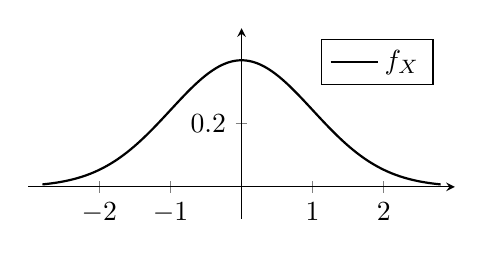
\begin{tikzpicture}
    \begin{axis}[
        axis lines=middle,
        xmin=-3, xmax=3,
        ymin=-0.1, ymax=0.5,
        samples=200,
        domain=-2.8:2.8,
        width=7cm,
        height=4cm,
        xtick={-2, -1, 0, 1, 2},
        ytick={0.2},
        yticklabels={0.2},
        legend style={at={(0.95,.7)}, anchor=south east},
    ]

    % density
    \addplot[thick] {
        exp(-x^2/2)/(sqrt(2*pi))
    };
    \addlegendentry{$f_X$}
    \end{axis}
\end{tikzpicture}
    }
    \caption{Standard normal density \(f_X\) from \eqref{eq: standard normal density}}
\end{wrapfigure} 
We will now characterize the asymptotic distribution of the rescaled mean using
Lévy's continuity theorem. With the benefit of historical hindsight we already
know that the limiting distribution is the normal distribution so we start
with its definition and the calculation of its characteristic function.

\begin{definition}[Univariate normal distribution]
    \label{def: univariate normal distribution}
    A random variable \(X\) in \(\real\) is \textbf{standard normal
    distributed} if it has density
    \begin{equation}
        \label{eq: standard normal density}
        f_X(x)
        = \frac1{\sqrt{2\pi}}
        \exp\bigl(-\tfrac{x^2}{2}\bigr).
    \end{equation}
    A random variable \(X\) in \(\real\) is \textbf{normal
    distributed} with mean \(\mu \in \real\) and variance \(\sigma^2 \mathop{\red{\ge}} 0\),
    denoted \(X \sim \normal{\mu, \sigma^2}\), if one of the following
    equivalent conditions holds:
    \begin{enumerate}[label=(\roman*)]
        \item\label{it: standard normal} \(X \overset{d}= \mu + \sigma Y\) where \(Y\) is a \underline{standard normal} random variable,

        \item\label{it: mgf normal}
        % the moment generating function of \(X\) is given by
        \(
            \MGF_X(t)
            = \exp\bigl(\mu t + \tfrac12 \sigma^2 t^2\bigr),
        \)

        \item\label{it: char fct normal}
        %the characteristic function of \(X\) is given by
        \(
            \charFct_X(t)
            = \exp\bigl(i \mu t - \tfrac12 \sigma^2 t^2\bigr).
        \)
    \end{enumerate}
\end{definition}
\begin{remark}
    We do not require \(\sigma^2 > 0\) in the definition! However, if
    \(\sigma^2>0\), then by Exercise \ref{ex: density of normal distribution} \(X\sim \normal{\mu, \sigma^2}\) has density
    \[
        f_X(x) = \frac1{\sqrt{2\pi \sigma^2}}
        \exp\bigl(-\tfrac{(x-\mu)^2}{2\sigma^2}\bigr).
    \]
    This is usually taken as the definition of the normal distribution. However
    this definition does not work for \(\sigma^2=0\) and would prevent the
    central limit theorem to hold in this case. And the importance of the normal
    distribution is solely justified by the CLT. Moreover the multivariate normal
    distribution will be less awkward to define if we allow zero variance.
\end{remark}
\begin{proof}[Proof (Definition \ref{def: univariate normal distribution} is well defined)]
    We delay the proof that the density \eqref{eq: standard normal density} integrates to one
    to Lemma \ref{lem: standard normal density integrates to one}. The equivalence of the definitions of the
    normal distribution follows from a calculation of the moment generating and
    characteristic functions due to the uniqueness of these functions (Fact
    \ref{fact: uniqueness of mgf and char fct}). We start with the moment
    generating function. Assuming \ref{it: standard
    normal} we have
    \begin{equation}
        \label{eq: mgf normal calculation}    
        \MGF_X(t) = \MGF_{\mu + \sigma Y}(t) = \Exp{e^{t(\mu + \sigma Y)}} = e^{\mu t}\MGF_Y(\sigma t)
    \end{equation}
    and thus it suffices to calculate the moment generating function \(\MGF_Y\),
    \[
        \MGF_Y(t)
        = \int_\real \exp(tx) \frac1{\sqrt{2\pi}}
        \exp\bigl(-\tfrac{x^2}{2}\bigr) dx
        = \frac1{\sqrt{2\pi}} \int_\real
        \exp\Bigl(-\frac1{2}\bigl(x^2 - 2 tx\bigr)\Bigr) dx.
    \]
    The exponent may be brought into the form \((x-\tilde{\mu})^2 +
    c\), where the residual \(c\) is constant in \(x\).
    Specifically, we have
    \[
        x^2 - 2 tx
        = \bigl(x^2 - 2 t x + t^2 - t^2\bigr)
        = (x - t)^2 - t^2.
    \]
    Put back into the integral this yields
    \[
        \MGF_Y(t)
        = \exp\bigl(\tfrac12 t^2\bigr)
        \frac1{\sqrt{2\pi}} \int_\real
        \exp\bigl(-\tfrac1{2}(x - t)^2\bigr) dx
        = \exp\bigl(\tfrac12 t^2\bigr),
    \]
    and consequently by \eqref{eq: mgf normal calculation} \(\MGF_X(t) = e^{\mu t} e^{\frac12 \sigma^2 t^2}\).
    For the characteristic function observe that \(t\mapsto e^{\mu t + \frac12
    \sigma^2 t^2}\) is an entire analytic function on \(\complex\), it is the
    unique analytic continuation of \(\MGF_X\) to \(\complex\) and thus
    \(\charFct_X(t) = \MGF_X(it) = e^{i \mu t - \frac12 \sigma^2 t^2}\).
\end{proof}

We are finally ready to prove the univariate central limit theorem.

\begin{mdframed}[innertopmargin=0pt]
\begin{theorem}[Univariate CLT]
    \label{thm: univariate central limit theorem}
    Let \((X_n)_{n\in \nat}\) be iid copies of the random variable \(X\in
    \cL^2(\real)\) with mean \(\mu = \Exp{X}\) and variance \(\sigma^2 =
    \var{X}\). Then
    \[
        \sqrt{n}\bigl(\mean{X}_n - \mu\bigr)
        \overset{d}\to \normal{0, \sigma^2}.
    \]
\end{theorem}
\end{mdframed}

\begin{proof}
    Without loss of generality we may assume that \(m=0\) since we can
    consider the centered random variables \(\tilde{X}_n = X_n - m\).
    We then have
    \[
        \charFct_{\sqrt{n} \mean{X}_n}(t)
        = \Exp[\Big]{\exp\Bigl(i \frac{t}{\sqrt{n}} \sum_{k=1}^n X_k\Bigr)}
        = \prod_{k=1}^n \Exp{\exp\Bigl(i \tfrac{t}{\sqrt{n}} X_k\Bigr)}
        = \charFct_{X}(\tfrac{t}{\sqrt{n}})^n.
    \]
    Since second moments are finite, \(\Exp{X_1} = 0\) and \(\sigma^2 =
    \Exp{X_1^2}\), we have by the representation for characteristic functions
    (Lemma \ref{lem: characteristic function representation})
    \[
        \charFct_X(\tfrac{t}{\sqrt{n}})
        = \Biggl[\sum_{k=0}^2 \Exp{X^k}\frac{(i\frac{t}{\sqrt{n}})^k}{k!} + o\Bigl(\frac{t^2}{n}\Bigr)\Biggr]
        = 1 - \frac{\sigma^2 t^2}{2 n} + o\Bigl(\frac{t^2}{n}\Bigr).
    \]
    Consequently we have by Lemma \ref{lem: compound interest}
    \[
        \charFct_{\sqrt{n} \mean{X}_n}(t)
        = \Bigl(1 - \tfrac{\sigma^2 t^2}{2 n} + o(\tfrac{t^2}{n})\Bigr)^n
        \to e^{-\frac12 \sigma^2 t^2}.
    \]
    Since that is the characteristic function of a normal distribution
    with mean zero and variance \(\sigma^2\) (Definition \ref{def: univariate
    normal distribution}) the claim follows by Lévy's continuity theorem (Fact \ref{fact: levy continuity}).
\end{proof}

In the proof of the central limit theorem we used the compound interest
formula in the complex case. This is the following Lemma.

\begin{lemma}[Compound interest]
    \label{lem: compound interest} Let \((x_n)_{n\in \nat}\) be a sequence in \(\complex\)
    with \(x_n \to x\in \complex\). Then
    \[
        \lim_{n\to\infty} (1+\tfrac{x_n}n)^n = e^{x}.
    \]
\end{lemma}
\begin{proof}
    Note that \(\exp\) is injective on the domain \(B\coloneq\Set{x+iy\in \complex: \abs{y} < \pi}\)
    with range \(\complex\setminus \real_{\le 0}\). Since \(1+\frac{x_n}n \to
    1\) this term eventually enters \(\complex\setminus \real_{\le
    0}\). Using the (analytic) inverse \(\ln\) of \(\exp\) restricted to \(B\)
    we thus have for sufficiently large \(n\)
    \[
        (1 + \tfrac{x_n}n)^n
        = \exp\bigl(\ln(1 + \tfrac{x_n}n)\bigr)^n
        = \exp\bigl(n \ln(1 + \tfrac{x_n}n)\bigr)
        = \exp\Bigl(x_n \frac{\ln(1 + \tfrac{x_n}n)}{x_n/n}\Bigr).
    \]
    \vspace*{-2ex}
    \begin{mdframed}[innertopmargin=0pt,innerbottommargin=0pt,rightline=false,topline=false,bottomline=false]
    Here we have tacitly assumed that \(x_n \neq 0\). We may
    do this without loss of generality:
    If there are only finitely many \(n\) with \(x_n=0\), then
    simply pick \(n\) large enough. In the other case
    the subsequence \((x_{n_k})_{k\in \nat}\) with \(x_{n_k} = 0\) still
    converges to \(x\) and consequently \(x=0\). In this case
    we also have \(\exp(n \ln(1+x_{n_k})) = \exp(0)= \exp(x)\) so
    we have convergence for this subsequence. We therefore only need
    to prove convergence for the remaining \(x_n\).
    Thus \(x_n\neq 0\) without loss of generality.
    \end{mdframed}
    Due to continuity it is sufficient to prove \(\frac1\lambda\ln(1 +
    \lambda) \to 1\) as \(\lambda \to 0\), where we choose \(\lambda = \frac{x_n}n\). Since the logarithm is analytic
    (complex differentiable)
    at \(1\) we however have
    \[
        \lim_{\lambda \to 0} \frac{\ln(1 + \lambda)}{\lambda}
        = \lim_{\lambda \to 0} \frac{\ln(1 + \lambda) - \ln(1)}{\lambda}
        = \ln'(1)
        = 1. \qedhere
    \]
\end{proof}

Since the normal distribution is the limit of sums, it is natural that the
distribution is stable under addition.

\begin{lemma}[Sum stability of normal distribution]
    \label{lem: sum stability of normal distribution}
    Let \(X_1,\dots, X_n\) be independent, normal random variables with \(X_i
    \sim \normal{\mu_i, \sigma_i^2}\). Then
    \[
        S_n \coloneq \sum_{i=1}^n X_i \sim \normal[\bigg]{\sum_{i=1}^n \mu_i,\; \sum_{i=1}^n \sigma_i^2}.
    \]
\end{lemma}
\begin{proof}
    We simply calculate the moment generating function using independence:
    \[\begin{aligned}[b]
        \MGF_{S_n}(t)
        &= \Exp[\Big]{\exp\Bigl(t \sum_{i=1}^n X_i\Bigr)}
        \overset{\text{indep.}}= \prod_{i=1}^n \MGF_{X_i}(t)
        = \prod_{i=1}^n \exp\bigl(\mu_i t + \tfrac12 \sigma_i^2 t^2\bigr)
        \\
        &= \exp\Bigl(t \sum_{i=1}^n \mu_i + \tfrac12 t^2 \sum_{i=1}^n \sigma_i^2\Bigr).
    \end{aligned}
    \qedhere
    \]
\end{proof}

\begin{remark}[Infinitely divisible distributions]
    Let \(X_1, X_2, \dots\) be iid random variables.  If the distribution of the
    sum is the same as an individual summand \(X_i\) up to location and scaling,
    that is
    \[
        X_1 + \dots + X_n \overset{d} = a_n X_1 + b_n,
    \]
    then the distribution of \(X_i\) is called \textbf{stable}. Since 
    the limit in \(n\) must still have this distribution, the CLT means that the
    normal distribution is the \emph{only} distribution with finite variance
    that has this property with \(a_n = n^{1/2}\). Fact: Without loss of generality the scaling can
    always be chosen to be of the form \(a_n = n^{1/\alpha}\) \citep[Thm.~16.22]{klenkeProbabilityTheoryComprehensive2014}.
    And for every \(\alpha\in (0, 2]\) there is exactly one stable distribution,
    the \(\alpha\)-stable distribution. The normal distribution is thus the
    only \(2\)-stable distribution. For \(\alpha\in (0,2)\) the tails
    decay according to a power law, roughly
    \[
        \Prob{\abs{X} >t} \sim t^{-\alpha} \qquad t\to \infty.
    \]
    Any distribution that is the limit of rescaled iid sums must be
    \(\alpha\)-stable. This can be seen by grouping the summands into \(n\)
    block of increasing size and observing that each block converges. Thus the
    sum of blocks has the same distribution as the original sum up to location
    and scale. A different name for \(\alpha\)-stable distributions are the
    ``infinitely divisible distributions'' since they can always be written as
    the sum of an arbitrary number of iid random variables. Being the limit of
    sums and being stable are thus equivalent concepts.
\end{remark}

\subsection{The Multivariate Central Limit Theorem}
\marginpar{\red{Lecture 5}}

For the multivariate central limit theorem we need to introduce the multivariate
normal distribution. To do so we require the concept of covariance matrices.

\begin{definition}[Covariance matrix]
    Let \(X, Y\) be random variables in \(\real^\dims\) with finite second moments.
    The \textbf{mixed covariance matrix} of \(X\) and \(Y\) is given by
    \[
        \Cov{X;Y}
        = \Exp[\Big]{\bigl(X - \Exp{X}\bigr)\bigl(Y - \Exp{Y}\bigr)^\top}
        \in \real^{\dims \times \dims}.
    \]
    Recall that the expectation is applied entrywise (Remark \ref{rem: expectation in multiple dimensions}).
    We write \(\Cov{X} \coloneq \Cov{X;X}\) for the \textbf{covariance matrix} of \(X\).
\end{definition}
\begin{remark}[Exercise \ref{ex: covariance matrix}]
    The covariance defined in Definition \ref{def: covariance and variance
    definition} is the trace of this covariance matrix, that is \(\tr\Cov{X;Y} =
    \cov{X}{Y}\) and the mixed covariance matrix is simply a corner of the
    covariance matrix of the vector \((X,Y)\), that is
    \[
        \Cov{X,Y} \coloneq \Cov{(X,Y)} = \begin{pmatrix}
            \Cov{X} & \Cov{X;Y} \\
            \Cov{Y;X} & \Cov{Y}
        \end{pmatrix}.
    \]
\end{remark}

\begin{lemma}[Covariance matrices are positive semidefinite]
    \label{lem: covariance matrix psd}
    Let \(X\) be a random variable in \(\real^\dims\) with covariance matrix
    \(\Sigma = \Cov{X}\). Then \(\Sigma\) is \underline{symmetric} and
    \underline{positive semidefinite}, that is \(\Sigma = \Sigma^\transpose\)
    and \(\inner{v, \Sigma v} \ge 0\) for all \(v\in \real^\dims\).
\end{lemma}
\begin{proof}
    The expectation is applied entrywise and as \(Y Y^\transpose\) is always
    symmetric this holds in particular for \(Y\coloneq (X - \Exp{X})\).
    To see positive semidefiniteness observe that for any \(v\in \real^\dims\)
    \[
        v^\transpose \Sigma v = \Exp[\big]{v^\transpose Y Y^\transpose v}
        = \Exp{\inner{Y, v}^2} \ge 0.
        \qedhere
    \]
\end{proof}
\begin{remark}[Variance interpretation]
    Positive semidefiniteness has the interpretation that all linear
    combinations \(\inner{v, X}\) of \(X\) have non-negative variance, because
    due to \(\inner{Y, v} = \inner{X, v} - \Exp{\inner{X,v}}\) we have
    \[
        v^\transpose \Sigma v
        = \Exp{\inner{Y, v}^2}
        = \var{\inner{X, v}}.
    \]
\end{remark}

\begin{remark}[Non-negative eigenvalue interpretation]
    Recall from Linear Algebra that a symmetric matrix always admits an
    eigenvalue decomposition with orthogonal eigenvectors and real eigenvalues.
    That is \(\Sigma = U \CGF U^\transpose\), where the columns of
    the orthonormal matrix \(U\) are the orthonormal eigenvectors \(u_i\) and
    the eigenvalues \(\lambda_i\) are the entries of the diagonal matrix
    \(\CGF\). Thus all eigenvalues of a positive semidefinite matrix
    are non-negative since
    \[
        0\le u_i^\transpose \Sigma u_i = \lambda_i \|u_i\|^2 = \lambda_i.
    \]
\end{remark}

\begin{definition}[Multivariate normal distribution]
    \label{def: multivariate normal distribution}
    Let \(\mu\in \real^\dims\) and \(\Sigma \in \real^{\dims \times \dims}\)
    be a symmetric \underline{positive semidefinite} matrix.
    A random variable \(X\) in \(\real^\dims\) is \textbf{multivariate normal
    distributed} with mean \(\mu\) and covariance \(\Sigma\), denoted by \(X
    \sim \normal{\mu, \Sigma}\), if one of the following equivalent conditions
    holds:
    \begin{enumerate}[label=(\roman*), noitemsep]
        \item\label{it: multivariate standard normal} \(X \overset{d}= \mu + A
        Y\) where \(Y=(Y^{(1)}, \ldots, Y^{(k)})\) is a vector of
        independent \underline{standard normal} random variables and
        \(A\in \real^{\dims\times k}\) satisfies \(A A^\transpose = \Sigma\),

        \item\label{it: multivariate linear normal}
        \(\inner{t, X} \sim \normal[\big]{\inner{t, \mu}, \inner{t, \Sigma t}}\)
        for all \(t\in \real^\dims\),

        \item\label{it: multivariate mgf normal}
        \(
            \MGF_X(t)
            = \exp\bigl(\inner{\mu, t} + \tfrac12 \inner{t, \Sigma t}\bigr),
        \)

        \item\label{it: multivariate char fct normal}
        \(
            \charFct_X(t)
            = \exp\bigl(i \inner{\mu, t} - \tfrac12 \inner{t, \Sigma t}\bigr).
        \)
    \end{enumerate}
\end{definition}

\begin{remark}[Strict positive definite]
    If \(\Sigma\) is strictly positive definite, that is one of the following
    equivalent conditions holds:
    \begin{enumerate}[label={(\roman*)},noitemsep]
        \item \(\inner{v, \Sigma v} > 0\) for all \(v\neq 0\)
        \item all eigenvalues \(\lambda_i\) of \(\Sigma\) are strictly positive
        \item \(\Sigma\) is invertible
        \item \(\det(\Sigma) > 0\),
    \end{enumerate}
    then by Exercise \ref{ex: density of normal distribution} \(X\sim \normal{\mu, \Sigma}\) has density
    \[
        f_X(x)
        = \frac1{\sqrt{(2\pi)^\dims \det(\Sigma)}}
        \exp\Bigl(-\tfrac12 \inner[\big]{x - \mu, \Sigma^{-1}(x - \mu)}\Bigr).
    \]
    The interpretation of the case \(v^\transpose \Sigma v = 0\) is that the
    linear combination \(\inner{v,X}\) of \(X\) has zero variance. While
    \(\sigma^2=0\) seems like a degenerate case that may be avoided, trying to
    avoid that any linear combination has zero variance is much more awkward.
\end{remark}
\begin{proof}[Proof (Definition \ref{def: multivariate normal distribution} is well defined)]
    We will first show that for any symmetric positive semidefinite matrix \(\Sigma\)
    there exists a matrix \(A\) with \(A A^\transpose = \Sigma\),
    specifically we may choose \(A = U \CGF^{1/2}\) using the
    eigenvalue decomposition \(\Sigma = U \CGF U^\transpose\).
    Thus \ref{it: multivariate standard normal} is well defined for
    any symmetric positive semidefinite \(\Sigma\).
    Next we show that \ref{it: multivariate standard normal} implies 
    \ref{it: multivariate linear normal}. As
    \[
        \inner{t, X}
        \overset{d}= \inner{t, \mu + A Y}
        = \inner{t, \mu} + \inner{A^\transpose t, Y}
        = \inner{t, \mu} + \sum_{i=1}^k (A^\transpose t)^{(i)} Y^{(i)},
    \]
    Since the \(Y^{(i)}\) are independent standard normal random variables, we have that
    all their functions \(\sigma_i Y^{(i)}\) with \(\sigma_i \coloneq (A^\transpose t)^{(i)}\)
    are independent. By definition of the univariate normal distribution
    we moreover have \(\sigma_i Y^{(i)} \sim \normal{0, \sigma_i^2}\). Since
    \(\inner{t, X}\) is deterministic it is also independent from the rest and
    may be viewed as a normal random variable with zero variance. Consequently
    we have by the stability of the normal distribution under addition (Lemma \ref{lem: sum stability of normal distribution})
    that \(\inner{t, X} \sim \normal{\inner{t, \mu}, \sum_{i=1}^k \sigma_i^2}\).
    Finally, we have
    \[
        \sum_{i=1}^k \sigma_i^2
        = \sum_{i=1}^k \bigl((A^\transpose t)^{(i)}\bigr)^2
        = \|A^\transpose t\|^2
        = \inner{t, A A^\transpose t}
        = \inner{t, \Sigma t}.
    \]
    Finally, we calculate the moment generating and characteristic functions
    function and characteristic function from \ref{it: multivariate linear
    normal}. This concludes the proof with the uniqueness of these functions
    (Fact \ref{fact: uniqueness of mgf and char fct}). We have that
    \[
        \MGF_X(t) = \Exp{\exp(\inner{t, X})}
        = \MGF_{\inner{t, X}}(1)
        = \exp\bigl(\inner{t, \mu} + \tfrac12 \inner{t, \Sigma t}\bigr),
    \]
    using \(\inner{t, X} \sim \normal{\inner{t, \mu}, \inner{t, \Sigma t}}\)
    and the moment generating function of the univariate normal distribution.
    We get the characteristic function with the same trick.
\end{proof}

\begin{mdframed}[innertopmargin=0pt]
\begin{theorem}[Central Limit Theorem]
    \label{thm: central limit theorem}
    Let \((X_n)_{n\in \nat}\) be independent copies of the random variable
    \(X\in \cL^2(\real^\dims)\) with mean \(\mu = \Exp{X}\) and covariance matrix
    \(\Sigma = \Cov{X}\). Then
    \[
        \sqrt{n}\bigl(\mean{X}_n - \mu\bigr)
        \overset{d}\to \normal{0, \Sigma}.
    \]
\end{theorem}
\end{mdframed}
\begin{proof}
    We will deduce the multivariate central limit theorem from the univariate
    central limit theorem using Cramér-Wold (Corollary \ref{cor: cramer wold}).
    Let \(t\in \real^\dims\), then
    \[
        \inner[\big]{t, \sqrt{n}(\mean{X}_n - \mu)}
        = \inner[\Big]{t, \frac1{\sqrt{n}} \sum_{k=1}^n X_k - \mu}
        = \frac1{\sqrt{n}}\sum_{k=1}^n \bigl(\inner{t, X_k} - \inner{t, \mu}\bigr)
    \]
    Since the \(\inner{t, X_k}\) are independent univariate copies of the random
    variable \(\inner{t, X}\) with mean \(\inner{t, \mu}\) and variance
    \[
        \var{\inner{t,X}}
        = \Exp{\inner{t, X - \mu}^2}
        = \Exp{t^\transpose (X - \mu)(X - \mu)^\transpose t}
        = t^\transpose \Sigma t,
    \]
    we may apply the univariate central limit theorem (Theorem \ref{thm: univariate central limit theorem})
    to obtain
    \[
        \inner{t, \sqrt{n}(\mean{X}_n - \mu)}
        \overset{d}\to \normal{0, t^\transpose \Sigma t}.
    \]
    The claim follows by Cramér-Wold (Corollary \ref{cor: cramer wold}).
\end{proof}

\begin{remark}[CLT in infinite dimension]
    Since Lévy's continuity theorem (Fact \ref{fact: levy continuity}) does
    not hold in infinite dimension it is more difficult to prove CLTs
    in infinite dimensional spaces (e.g.\ function spaces). The typical
    approach is to prove convergence of all finite dimensional projections
    (by the multivariate CLT) and prove that the sequence of distributions
    is in a compact set. This shows that any sequence has a converging
    subsequence. If the limit of every subsequence is the same, then we get
    convergence. But since the finite dimensional projections of every
    subsequence still converge to the same limit it is possible to
    identify the limit uniquely.
\end{remark}


\subsection{Special properties of the normal distribution}

\begin{remark}[Uncorrelated \textbf{kind of} implies independent]
    If \(X\) is a multivariate normal random vector and its components are
    uncorrelated, then its covariance \(\Cov{X}\) is diagonal.
    In Exercise \ref{ex: density of normal distribution} you will show
    that \(\Sigma = \Cov{X}\) and consequently, \(\Sigma\) is diagonal
    with entries \(\sigma_1^2, \ldots, \sigma_\dims^2\).
    Choosing \(A = \diag[\sigma_1, \ldots, \sigma_\dims]\)
    we have \(AA^\transpose = \Sigma\) and thus by Definition
    \[
        X \overset{d}= \mu + A Y = \begin{pmatrix}
            \mu^{(1)} + \sigma_1 Y^{(1)} \\
            \vdots \\
            \mu^{(\dims)} + \sigma_\dims Y^{(\dims)}
        \end{pmatrix}
    \]
    Thus every \(X^{(i)}\) is a function of only \(Y^{(i)}\) and since the
    \(Y^{(i)}\) are independent, the \(X^{(i)}\) are independent as well.

    \textbf{However}, if \(X\) and \(Y\) are both normal distributed but
    \((X,Y)\) is not a multivariate normal random vector, then uncorrelatedness
    does not imply independence in general (see Exercise \ref{ex: uncorrelated
    but not independent normal}).
\end{remark}

\begin{fact}[Herschel-Maxwell characterization]
    Let \(X\) be a random vector in \(\real^\dims\) with independent components
    \(X^{(i)}\). Further assume \(X\) has rotation invariant distribution, that is
    for all orthogonal \(U\in \real^{\dims\times \dims}\)
    \[
        X \overset{d}= U X.
    \]
    Then necessarily \(X\sim \normal{0, \sigma^2 \identity}\) for some \(\sigma^2 \ge 0\).
\end{fact}
\begin{proof}[Proofsketch]
    Let \(\dims=2\). By rotation invariance both components \(X^{(1)}\) and
    \(X^{(2)}\) are are identically distributed. Thus the components are iid. If
    they have a density \(f\), then the joint density factorizes, that is
    \[
        f_X(x_1, x_2) = f(x_1) f(x_2)
    \]
    Due to rotation invariance the joint density must only depend on the
    radius, or equivalently squared radius \(\|x\|^2 = x_1^2 + x_2^2\).
    Thus it must be of the form
    \[
        f_X(x_1, x_2) = g(x_1^2 + x_2^2)
    \]
    Setting \(x_2=0\) we observe by the two expressions \(g(x_1^2) = f(x_1)f(0)\).
    Thus
    \[
        g(x_1^2 + x_2^2) = f(x_1) f(x_2) = \frac{g(x_1^2)}{f(0)} \frac{g(x_2^2)}{f(0)}.
    \]
    The only functions \(g\) that satisfy \(g(x+y) = \frac1c g(x) g(y)\) are \(x\mapsto c\exp(\lambda x)\)
    for \(\lambda\in \real\). Thus
    \[
        f(x_1) = \frac{g(x_1^2)}{f(0)} = \frac{c}{f(0)} \exp(\lambda x_1^2)
        = f(0) \exp(\lambda x_1^2).
    \]
    Since the density must integrate to one we rule out \(\lambda \ge 0\) and
    arrive at the normal distribution. An actual proof would
    however need to justify the existence of a density.
\end{proof}

In light of this rotation invariant characterization the following proof that
the normal distribution is a density is perhaps less surprising:

\begin{lemma}[Standard normal density integrates to one]
    \label{lem: standard normal density integrates to one}
    The density of the standard normal distribution integrates to one, that is
    \[
        I \coloneq \int \exp\bigl(-\tfrac{x^2}{2}\bigr) dx = \sqrt{2\pi}.
    \]
\end{lemma}
\begin{proof}
We will show that $I^2=2\pi$. We observe that
\begin{align*}
I\times I ={} & 
\left(\int_{-\infty}^{\infty} \exp\left(-\frac{x^2}{2}\right) \mathrm{d}x \right)
\left(\int_{-\infty}^{\infty} \exp\left(-\frac{y^2}{2}\right) \mathrm{d}y \right)\\
={} & 
\int_{-\infty}^{\infty}
\int_{-\infty}^{\infty}
\exp\left(-\frac{x^2+y^2}{2}\right) \mathrm{d}x\mathrm{d}y
\end{align*}
Here the squared radius \(r^2 = x^2 + y^2\) appears naturally in the exponent.
We evaluate this integral using polar coordinates. We change variables from $(x,y)$ to $(r,\theta)$ by using the transformation
\[
    x \coloneqq r \cos\theta, \qquad y \coloneqq r \sin\theta.
\]
The Jacobian determinant of this transformation is
\[
\left|\begin{pmatrix}
\frac{\partial x}{\partial r} & \frac{\partial y}{\partial r} \\
\frac{\partial x}{\partial \theta} & \frac{\partial y}{\partial \theta} \\
\end{pmatrix}\right| 
= \left|\begin{pmatrix}
\cos\theta & \sin\theta \\
-r\sin\theta & r\cos\theta \\
\end{pmatrix}\right| = r(\cos^2\theta + \sin^2\theta) = r\;.
\]
Therefore,
\[
I\times I = 
\int_{0}^\infty \int_{0}^{2\pi} e^{-\frac{r^2}{2}} \, r \, \mathrm{d}\theta \mathrm{d}r = 
2\pi \int_0^\infty e^{-\frac{r^2}{2}} \, r \, \mathrm{d}r 
= 2\pi \left[-e^{-\frac{r^2}{2}}\right]_{0}^{\infty}
=  2\pi \;.
\qedhere
\]
\end{proof}

\subsection*{Exercises}

\begin{exercise}[Properties of moment generating functions]
    \label{ex: properties moment generating functions}
    Let \(X, Y\) be random variables in a Hilbert space \(\hilbert\).
    Then
    \begin{enumerate}[label=(\alph*)]
        \item \(\MGF_X(0) = 1\).
        \item \(\MGF_{aX + b}(h) = e^{\inner{h,b}} \MGF_X(a h)\)
        for any \(a\in \real\), \(b, h\in \hilbert\),
        \item \(\MGF_{X+Y}(h) = \MGF_X(h) \MGF_Y(h)\) for \(X,Y\) independent and all \(h\in \hilbert\).
    \end{enumerate}
    Similarly we have for the characteristic function
    \begin{enumerate}[label=(\alph*), resume]
        \item \(\abs{\charFct_X(t)}\le 1\) and \(\charFct_X(0) = 1\).
        \item \(\charFct_{X+Y}(t) = \charFct_X(t) \charFct_Y(t)\) for \(X,Y\) independent and all \(t\in \hilbert\).
        \item \(\charFct_{aX + b}(t) = e^{i\inner{t,b}} \charFct_X(a t)\)
        for any \(a\in \real\), \(b, t\in \hilbert\).
    \end{enumerate}
\end{exercise}

\begin{exercise}[Moment generating functions]
    Prove the formulas for the moment generating functions in the following
    table
    \begin{center}
    \def\arraystretch{1.5}
    \begin{tabular}{l l l}
        \(\Pr_X\)
        &  \(\MGF_X(t)\) & \(\charFct_X(t)\)
        \\
        \hline
        \(\normal{\mu, \sigma^2}\) & \(e^{\mu t + \frac12 \sigma^2 t^2}\)
        & \(e^{i \mu t - \frac12 \sigma^2 t^2}\)
        \\
        \(\bernoulli(p)\) & \(1 - p + p e^{t}\)
        & \(1 - p + p e^{i t}\)
        \\
        \(\Binomial(n, p)\) & \((1 - p + p e^{t})^n\)
        & \((1 - p + p e^{i t})^n\)
        \\
        \(\exponential(\lambda)\) & \(\frac{\lambda}{\lambda - t}\) for \(t < \lambda\)
        & \(\frac{\lambda}{\lambda - i t}\)
        \\
        \(\Poisson(\lambda)\) & \(e^{\lambda (e^{t} - 1)}\)
        & \(e^{\lambda (e^{i t} - 1)}\) 
    \end{tabular}
    \end{center}
\end{exercise}

\begin{exercise}[The normal distribution]
    \label{ex: density of normal distribution}
    Let \(X \sim \normal{\mu, \sigma^2}\).
    \begin{enumerate}[label=(\alph*)]
        \item 
        Show that if \(\sigma^2 > 0\), then \(X\) has density
        \[
            f_X(x) = \frac1{\sqrt{2\pi \sigma^2}}
            \exp\bigl(-\tfrac{(x-\mu)^2}{2\sigma^2}\bigr).
        \]
        \begin{solution}
            We show that the distribution of \(Z = \mu + \sigma Y\) is equal to a random variable \(X\)
            with density \(f_X\). Let \(g\) be a bounded continuous function, then we
            have
            \[\begin{aligned}
                \Exp{g(Z)}
                &= \Exp{g(\mu + \sigma Y)}
                \\
                &= \int_\real g(\mu + \sigma y) \frac1{\sqrt{2\pi}} \exp\bigl(-\tfrac{y^2}2\bigr) dy
                \\
                \overset{x=\mu + \sigma y}&=
                \int_\real g(x) \frac1{\sqrt{2\pi \sigma^2}} \exp\bigl(-\tfrac{(x-\mu)^2}{2\sigma^2}\bigr) dx
                \qquad\quad ``\tfrac{1}{\sigma} dx =  dy''
                \\
                &= \Exp{g(X)}.
            \end{aligned}
            \]
            Since this is true for all bounded continuous functions \(g\) we have \(X \overset{d}= Z\).
            Consequently the density of \(Z\) is given by \(f_X\).
        \end{solution}

        \item Calculate all the moments \(\Exp{X^n}\) of \(X\).

        \item Show that \(\Exp{X} = \mu\) and \(\var{X} = \sigma^2\).
    \end{enumerate}
    Let \(X \sim \normal{\mu, \Sigma}\) be a multivariate normal random variable.
    \begin{enumerate}[label=(\alph*), resume]
        \item Show that if \(\Sigma\) is strictly positive definite, then \(X\) has density
        \[
            f_X(x)
            = \frac1{\sqrt{(2\pi)^\dims \det(\Sigma)}}
            \exp\Bigl(-\tfrac12 \inner[\big]{x - \mu, \Sigma^{-1}(x - \mu)}\Bigr).
        \]
        
        \item Prove that \(\Exp{X} = \mu\) and \(\Cov{X} = \Sigma\).

        \item Assume that \(\Sigma\) is not positive semidefinite, that is
        \(v \Sigma v < 0\) for some vector \(v\) prove that there is no random
        variable \(X\) with characteristic function
        \[
            \charFct_X(t)
            = \exp\bigl(i \inner{\mu, t} - \tfrac12 \inner{t, \Sigma t}\bigr).
        \]
        \textbf{Hint:} \eqref{eq: bound on characteristic function}.
    \end{enumerate}

\end{exercise}


\begin{exercise}[Multivariate moment generating function]
    \label{ex: multivariate moment generating function}
    Let \(X\) be a random vector in \(\real^d\) with \(\MGF_X(t) < \infty\)
    for all \(h\in \ball{0}{r}\) for some radius \(r > 0\). Show that all mixed moments
    \(\Exp{\abs{X_1^{k_1} \cdots X_d^{k_d}}}\) exist and
    \[
        \MGF_X(h) = \sum_{k=0}^\infty \frac{\Exp{\inner{h, X}^k}}{k!}
        = \sum_{k_1, \dots, k_d = 0}^\infty
        \Exp{X_1^{k_1} \cdots X_d^{k_d}}
        \frac{h_1^{k_1} \cdots h_d^{k_d}}{k_1! \cdots k_d!}.
    \]
\end{exercise}

\begin{exercise}[Lévy's continuity theorem in infinite dimensions]
    \label{ex: counterexample levy's continuity in infinite dim}
    To show that Lévy's continuity theorem does not hold in infinite dimensions
    consider the deterministic sequence \(X_n = e^n\), where \(e^n=(0,\dots,0, 1, 0, \dots)\) is the
    \(n\)-th unit vector in the Hilbertspace of square summable sequences 
    \[
        \ell^2 = \Set[\Big]{(x_n)_{n\in \nat} \mid \sum_{n=1}^\infty x_n^2 < \infty}
        \qquad\text{with}\qquad
        \inner{x, y} = \sum_{n=1}^\infty x_n y_n.
    \]
    Let \(X=0\in \ell^2\) be the deterministic zero vector. Show that
    \begin{enumerate}[label=(\alph*), noitemsep]
        \item \(\charFct_{X_n}(h) \to \charFct_{X}(h)\) for all \(h\in \ell^2\),
        \item \(X_n \not\overset{d}\to X\).
    \end{enumerate}
\end{exercise}

\begin{exercise}[Uncorrelated but not independent normal]
    \label{ex: uncorrelated but not independent normal}
    Let \(Z \sim \normal{0,1}\) and \(\epsilon \sim \uniform(\Set{-1,1})\) be independent
    random variables and define
    \[
        X = Z, \qquad Y = \epsilon Z.
    \]
    Show that \(X\) and \(Y\) are both normal distributed and uncorrelated but not independent.
\end{exercise}

\begin{exercise}[Covariance matrices]
    \label{ex: covariance matrix}
    For \(X \in \cL^2(\real^\dims)\) and \(Y \in \cL^2(\real^{\dims'})\) Show
    that
    \begin{enumerate}[label=(\alph*), noitemsep]
        \item for \(\dims = \dims'=1\) we have \(\Cov{X;Y} = \Cov{Y;X} = \cov{X}{Y}\).
        \item the covariance matrix \(\Cov{X}\) is symmetric and may be written as
        \[
            \Cov{X} 
            = \begin{pmatrix}
                \Cov{X_1;X_1} & \cdots & \Cov{X_1;X_d} \\
                \vdots & \ddots & \vdots \\
                \Cov{X_d;X_1} & \cdots & \Cov{X_d;X_d}
            \end{pmatrix}
        \]

        \item \(\cov{X}{Y} = \tr\Cov{X;Y}\).

        \item the mixed covariance matrix is the corner of the concatenated
        covariance matrix, that is
        \[
            \Cov{X,Y} \coloneq \Cov{(X,Y)} = \begin{pmatrix}
                \Cov{X} & \Cov{X;Y} \\
                \Cov{Y;X} & \Cov{Y}
            \end{pmatrix}.
        \]

    \end{enumerate}
\end{exercise}

\section{Large Deviations and concentration inequalities}
\label{sec: concentration inequalities}

In the previous section was concerned with the distribution of \emph{typical deviations} of
the mean, which were of order \(\frac1{\sqrt{n}}\). The purpose of this section is two-fold. First, we want to understand
how fast the probability of \emph{large deviations} of constant order \(1\) decay with \(n\).
Second, we want more quantitative bounds on the deviation probability.
Observe that the central limit theorem only gives an asymptotic statement:
``If \(n\to\infty\), then...''. However in practice \(n\) is always finite.
And we can never be sure that the normal distribution is really a good
approximation of the distribution at finite \(n\).
\begin{quotation}
    ``In the long run we are all dead'' -- John Maynard Keynes 
\end{quotation}
It is a lucky coincidence that the tools to analyze large deviations are also
better suited to provide quantitative bounds. Quantitative versions of the CLT
also exist, but they come at the price of much greater difficulty.

With a quantitative bound we mean that we want an explicit upper bound
\[
    \Prob[\big]{\norm{X_n - X} \ge \epsilon} \le \delta
\]
for a fixed \(n\) instead of just the statement that this probability goes to zero as
\(n\to\infty\). Such statements are also know as ``probably, approximately
correct'' (PAC) statements, that is
\begin{quote}
``with probability at least \(1-\delta\) (probably), we have \(\norm{X_n - X} <
\epsilon\) (approximately) for a specific \(n\in \nat\)''.
\end{quote}

\subsection{A real valued introduction}

Recall that the only tool we have used so far to bound probabilities is the
Markov inequality (Theorem \ref{thm: markov inequality})
\[
    \Prob{ X \ge a} \le \tfrac{\Exp{h(X)}}{h(a)}.
\]
The choice \(h(x) = e^{tx}\), with \(t\ge 0\) such that \(h\) is
non-decreasing, results in the ``\textbf{Chernoff bound}''
\[
    \Prob{X \ge a}
    \le \frac{\Exp{e^{t  X}}}{e^{t a}}
    = \frac{\MGF_X(t)}{e^{t a}}
    = \exp\bigl(-\bigl(t a - \underbrace{\log \MGF_X(t)}_{=\CGF_X(t)}\bigr)\bigr).
\]
If the moment generating function of \(X\) is not finite, then this bound is
of course useless. Note that we cannot use the characteristic function here,
since the Markov inequality requires non-negative, and in particular
real-valued, functions \(h\). The function \(\CGF_X\) is the ``\textbf{cumulant
generating function}'' (CGF) or ``log-laplace transform'' that will be our main object
of study in this section.

The key feature of the Chernoff bound is that it provides us with a parameter \(t\)
that is not inherent to the problem of bounding \(\Prob{X \ge a}\). This allows for
an optimization over \(t\), resulting in the \textbf{Legendre transform}
\[
    \CGF^+_X(a) \coloneq \sup_{t\ge 0} \bigl( t a - \CGF_X(t) \bigr).
\]
The optimized bound is then given by
\begin{equation}
    \label{eq: chernoff bound}    
    \Prob{X \ge a} \le \exp\bigl(-\CGF^+_X(a)\bigr).
\end{equation}

\begin{example}[The normal distribution]
    Let \(X \sim \normal{\mu, \sigma^2}\). 
    Recall that the moment generating function of the normal distribution was
    \(\MGF_X(t) = \exp(\mu t + \frac12 \sigma^2 t^2)\) (Definition \ref{def:
    univariate normal distribution}). Its CGF is then given by the quadratic
    polynomial
    \[
        \CGF_X(t) = \mu t + \tfrac12 \sigma^2 t^2.
    \]
    Thus the Legendre transform is
    \[\begin{aligned}
        \CGF_X^+(a)
        = \sup_{t\ge 0} \bigl(t a - \mu t - \tfrac12 \sigma^2 t^2\bigr)
        &= \sup_{t\ge 0} \bigl(t (a - \mu) - \tfrac12 \sigma^2 t^2\bigr)
        \\
        &= \begin{cases}
        \frac{(a - \mu)^2}{2\sigma^2}
        \qquad &\text{for } a \ge \mu,
        \\
        0 &\text{for } a \le \mu.
        \end{cases}
    \end{aligned}\]
    The last step follows from simple optimization. The first order condition
    results in the aximizer \(t^\star = \frac{a - \mu}{\sigma^2}\), which is greater
    zero if and only if \(a \ge \mu\).
    Observe that if \(\CGF_X^+(a) = 0\), then the Chernoff bound \eqref{eq: chernoff bound}
    is \(1\) which is not very helpful since probabilities are always bounded by \(1\).
    The only useful case is thus \(a \ge \mu\), in which we get that
    the tail of the normal distribution decays like a squared exponential in the
    distance \((a-\mu)\) to the mean, that is
    \[
        \Prob{X \ge a}
        \le \exp\bigl(- \tfrac{(a - \mu)^2}{2\sigma^2}\bigr)
        \qquad\text{for } a \ge \mu.
    \]
    Or equivalently, with \(\epsilon = a - \mu > 0\) we get quickly decaying bound in \(\epsilon\)
    \[
        \Prob{X - \mu \ge \epsilon}
        \le \exp(-\tfrac{\epsilon^2}{2\sigma^2})
        \qquad\text{for } \epsilon \ge 0.
    \]
\end{example}

Since \(\CGF_X^+\) is defined as a supremum over all \(t\ge 0\), it does not
translate well into multiple dimension where the ordering is lost.
We have seen in the example above that the maximizer \(t^\star\) is positive
whenever \(a\ge \mu\) or equivalently \(\epsilon = a - \mu \ge 0\).
This implies that for \(a\ge \mu\) the function \(\CGF_X^+(a)\) coincides
with the \textbf{convex conjugate}, also known as ``Fenchel-Legendre transform''
of \(\CGF_X\) given by
\[
    \CGF_X^*(a) \coloneq \sup_{t\in \real} \bigl(t a - \CGF_X(t)\bigr)
    \qquad \Bigl(\ge \CGF_X^+(a)= \sup_{t \ge 0} \bigl(t a - \CGF_X(t)\bigr)\Bigr).
\]
\begin{warning}
    For \(a\le \mu\) the bound \(\Prob{X \ge a} \le \exp(-\CGF_X^*(a))\) is
    false! Here \(\CGF_X^*(a) > \CGF_X^+(a) = 0\).  However since
   \(\CGF_X^+(a)=0\) is a useless bound anyway, we simply need to avoid this
    case.
\end{warning}

% To understand the convex conjugate for \(a\le \mu\), observe that in this case
% \(-a \ge -\mu = \Exp{-X}\). Consequently,
% \[
% \begin{aligned}
%     \CGF_{-X}^+(-a)
%     = \sup_{t\ge 0} \bigl(t (-a) - \CGF_{-X}(t)\bigr)
%     &= \sup_{t\ge 0} \bigl(-ta - \CGF_{X}(-t)\bigr)
%     \\
%     &= \sup_{s\le 0} \bigl(sa - \CGF_{X}(s)\bigr)
%     = \CGF_X^*(a),
% \end{aligned}
% \]
% where we use \(\CGF_{-X}(t) = \log\Exp{e^{t(-X)}}= \CGF_X(-t)\).
% So in essence
% \begin{alignat}{3}
%     \Prob{X \ge a} &\le \exp\bigl(-\CGF_X^*(a)\bigr) &\text{for }a &\ge \mu,
%     \\ 
%     \Prob{X \le a} = \Prob{-X \ge -a} &\le \exp\bigl(-\CGF_{X}^*(a)\bigr)\qquad &\text{for } a &\le \mu.
% \end{alignat}
% Why is this useful? For \(a \le \mu \le b\) consider
% \[
%     \Prob{X \in (a,b)^\complement}
%     = \Prob{X \le a} + \Prob{X \ge b}
% \]

% For concentration bounds we will simply use
% \[\begin{aligned}
%     \Prob{\abs{X} \ge a}
%     &= \Prob{X \ge a} + \Prob{-X \ge a}
%     \\
%     &\le \exp\bigl(-\CGF^+_X(a)\bigr) + \exp\bigl(-\CGF^+_{-X}(a)\bigr)
% \end{aligned}\]

\subsection{Large Deviations}
\marginpar{\red{Lecture 6}}

With the motivation above let us now formalize this procedure in multiple dimensions.

\begin{definition}[Cumulant generating function]
    The \textbf{cumulant generating function} (CGF) of a random variable \(X\)
    in a Hilbertspace \(\hilbert\) is defined as the logarithm of its moment generating
    function
    \[
        \CGF_X(t) \coloneq \log \MGF_X(t)
        = \log \Exp{e^{\inner{t, X}}}.
    \]
    Note that since \(\exp(x) \ge 0\) the MGF is always defined but possibly infinite,
    and thus the CGF also always well defined but possibly infinite. We further
    define the functions
    \begin{align*}
        \tag{concave-convex function}
        \Phi_X(t, a) &\coloneq \inner{t, a} - \CGF_X(t)
        \\
        \tag{convex conjugate}
        \CGF_X^*(a) &\coloneq \sup_{t\in \hilbert} \Phi(t, a)
    \end{align*}
\end{definition}

Observe that \(\Phi_X\) is a concave-convex function if \(\CGF_X\) is convex,
which is the case (see Lemma \ref{lem: check sion's conditions} below).
The function \(\CGF_X^*\) is the convex conjugate of \(\CGF_X\), which entails a
lot of nice structure (Exercise \ref{ex: convex conjugate}).

\begin{proposition}
    \label{prop: general LDP upper}
    Let \(A\subseteq \hilbert\) be a \underline{compact convex} set, then 
    \[
        \Prob{X \in A} \le \exp\bigl(-\inf_{a\in A} \CGF_X^*(a)\bigr).
    \]
\end{proposition}
\begin{proof}
    Then
    \(
        \inner{t, x} - \inf_{a\in A} \inner{t, a} \ge 0
    \)
    for all \(x\in A\) and any \(t\in \hilbert\). Since \(e^\lambda \ge 1\)
    for all \(\lambda \ge 0\) we have
    \[\begin{aligned}
        \Pr[X \in A] = \Exp{\Indicator{X \in A}}
        &\le \Exp[\Big]{\exp\bigl(\inner{t, X} - \inf_{a\in A} \inner{t, a}\bigr)}
        \\
        &= \MGF_X(t)\exp\bigl(- \inf_{a\in A} \inner{t, a}\bigr) 
        \\
        &= \exp\Bigl(- \bigl(\inf_{a\in A} \inner{t, a}-\CGF_X(t)\bigr)\Bigr) 
        = \exp(- \inf_{a\in A} \Phi_X(t, a)).
    \end{aligned}
    \]
    Since this bound holds for any \(t\in \hilbert\) we have by Sion's
    minimax theorem (Fact \ref{fact: sion's minimax theorem}) and Lemma
    \ref{lem: check sion's conditions}
    \[\begin{aligned}[b]
        \Pr[X \in A]
        &\le \exp\Bigl(- \sup_{t \in \hilbert} \inf_{a\in A} \Phi_X(t, a)\Bigr)
        \\
        \overset{\text{Sion}}&=
        \exp\Bigl(- \inf_{a\in A} \sup_{t \in \hilbert} \Phi_X(t, a)\Bigr)
        = \exp\bigl(- \inf_{a\in A} \CGF_X^*(a)\bigr).
    \end{aligned}
    \qedhere
    \]
\end{proof}

\begin{fact}[Sion's minimax theorem {\citep[e.g.][]{komiyaElementaryProofSions1988}}]
    \label{fact: sion's minimax theorem}
    Let \(\cX\) be a \underline{compact convex} subset of a topological vectorspace and
    \(\cY\) a convex subset of a topological vectorspace. Let
    \(f \colon \cX \times \cY \to \real\) be a function such that
    \begin{enumerate}[label=(\roman*), noitemsep]
        \item for each \(y \in \cY\), \(f(\cdot, y)\) is upper semicontinuous and quasi-concave on \(\cX\),
        \item for each \(x \in \cX\), \(f(x, \cdot)\) is lower semicontinuous and quasi-convex on \(\cY\).
    \end{enumerate}
    Then
    \[
        \sup_{x \in \cX} \inf_{y \in \cY} f(x, y)
        = \inf_{y \in \cY} \sup_{x \in \cX} f(x, y);
    \]
\end{fact}

\begin{lemma}[Check Sion's conditions]
    \label{lem: check sion's conditions}
    \(\Phi(t, a) = \inner{t, a} - \CGF_X(t)\) satisfies the conditions of Sion's minimax theorem.
\end{lemma}
\begin{proof}
    The function \(\Phi_X\) is trivially continuous and convex in \(a\) since
    the inner product is continuous and linear in \(a\). We need to check that the cumulant generating function \(\CGF_X\) is
    \begin{enumerate}[label={(\roman*)}, nosep]
        \item lower semicontinuous
        \item convex
    \end{enumerate}
    Then the function \(\Phi_X\) is upper semicontinuous and concave in \(t\).
    Lower semicontinuity
    of \(\CGF_X\) follows from Fatou's lemma (measure theory):
    \[\begin{aligned}
        \liminf_{n\to \infty} \CGF_X(\lambda_n)
        &= \log \liminf_{n\to \infty} \Exp{\exp(\inner{\lambda_n, X})}
        \\
        \overset{\text{Fatou}}&\ge \log \Exp{\liminf_{n\to \infty} \exp(\inner{\lambda_n, X})}
        = \CGF_X(\lambda).
    \end{aligned}
    \]
    Convexity of \(\CGF_X\) follows from Hölder's inequality (Exercise \ref{ex: hölder's inequality}).
    Specifically, for any \(t, s\in \hilbert\) and any \(\alpha\in[0,1]\) we choose
    \(p = \frac1\alpha\) and \(q = \frac1{1-\alpha}\) such that \(\frac1p
    + \frac1q = 1\), then
    \[\begin{aligned}[b]
        \CGF_X(\alpha t + (1-\alpha) s)
        &= \log \Exp{e^{\inner{\alpha t + (1-\alpha) s, X}}}
        \\
        \overset{\text{Hölder}}&\le \log \Exp{(e^{ \alpha\inner{t, X}})^{p}}^{\frac1p} \Exp{(e^{(1-\alpha)\inner{s, X}})^{q}}^{\frac1q}
        \\
        \overset{p=\frac1\alpha}&= \log \Exp{e^{\inner{t, X}}}^{\alpha} \Exp{e^{\inner{s, X}}}^{1-\alpha}
        = \alpha \CGF_X(t) + (1-\alpha) \CGF_X(s).
    \end{aligned}
    \qedhere
    \]
\end{proof}

In finite dimensions we can extend Proposition \ref{prop: general LDP upper} to
\emph{closed} convex sets.

\begin{mdframed}[innertopmargin=0pt]
\begin{theorem}[Generalized Chernoff bound]
    \label{thm: chernoff bound in R^d}
    Let \(A\subseteq \real^\dims\) be a \underline{closed}, \underline{convex} set, then 
    \[
        \Prob{X \in A} \le \exp\bigl(-\inf_{a\in A} \CGF_X^*(a)\bigr).
    \]
\end{theorem}
\end{mdframed}
\begin{proof}
    Let \((K_n)_{n\in \nat}\) be an increasing sequence of convex compact sets
    with \(K_n \uparrow \real^\dims\) (this does not exist in infinite
    dimension!). Then by continuity of probability measures
    (Remark \ref{rem: continuity of probability})
    \[\begin{aligned}[b]
        \Pr[X\in A]
        &\le \lim_{n\to \infty} \Pr[X \in A \cap K_n] + \underbrace{\Pr[X \notin K_n]}_{\to 0}
        \\
        &\le \lim_{n\to \infty} \exp\bigl(- \inf_{a\in A \cap K_n} \CGF_X^*(a)\bigr)
        \le \exp\bigl(- \inf_{a\in A} \CGF_X^*(a)\bigr).
    \end{aligned}
    \qedhere
    \]
\end{proof}


Since they are closely related to the MGF, the CGF also interacts very well with
independent sums.

\begin{lemma}
    Let \(X_1, \ldots, X_n\) be independent copies of the random variable \(X\)
    and \(\mean{X}_n\) their mean, then
    \begin{equation}
        \label{eq: cumulant generating function of the mean}
        \CGF_{\mean{X}_n}(t) = n \CGF_X\bigl(\tfrac{t}n\bigr)
        \qquad\text{and}\qquad
        \CGF_{\mean{X}_n}^*(t) = n \CGF_X^*(t).
    \end{equation}
\end{lemma}
\begin{proof}
    \red{TODO}
    Since the cumulant generating function of the sum \(\sum_{i=1}^n X_i\)
    is \(n \CGF_X(t)\) by independence, \ref{it: cumulant independent sums} and
    the fact that the \(X_i\) are identically distributed, we have by the scaling property
    Consequently
    \[
        \CGF_{\mean{X}_n}^+(a)
        = \sup_{t\ge 0} \bigl(n \tfrac{t}n a - n \CGF_X(\tfrac{t}n)\bigr)
        \overset{s=\frac{t}n}= n \sup_{s\ge 0} \bigl(s a - \CGF_X(s)\bigr)
        = n \CGF_X^+(a).
        \qedhere
    \]
\end{proof}

This Lemma with the Chernoff bound Theorem \ref{thm: chernoff bound in R^d} implies
exponential concentration bounds for the mean. Specifically,
let \(X_1, \ldots, X_n\) be independent copies of the random variable \(X\) and
\(\mean{X}_n\) their mean. Then
\begin{equation}
    \label{eq: exponential concentration of the mean}
    \Prob{\mean{X}_n \ge a}
    \le \exp\bigl(-n \CGF_X^+(a)\bigr).
\end{equation}
Now if \(\CGF_X^+(a) > 0\), then the probability that the mean exceeds \(a\)
decays exponentially in \(n\). This would of course be weird if \(a \le \Exp{X}\)
so we would expect that \(\CGF_X^+(a) = 0\) for \(a \le \Exp{X}\). And this
should make us suspicious: Is \(\CGF_X^+(a) > 0\) true for any \(a\) or is this
bound useless?


\begin{fact}[Cramér]
    
\end{fact}

\begin{fact}[Gärtner Ellis]
    
\end{fact}

\subsection{Subgaussian random variables}

Subgaussian random variables have tails that decay at least as fast as the
Gaussian distribution. That is
\[
    \Prob{\abs{X} \ge t} \le 2 \exp\bigl(-\tfrac{t^2}{2\sigma^2}\bigr).
\]
An important example would be bounded random variables, since the probability 
that \(\abs{X} \ge t\) eventually drops to zero.
Unfortunately tail bounds like this do not interact
well with summation of random variables. We would therefore prefer bounds on the
CGF instead to get tight bounds on the convergence rate of the mean. We will
start by defining such bounds and find out later (Theorem \ref{thm: subgaussian
equivalences}) that this is actually equivalent to the tail bound above in some
sense.

\begin{definition}[Variance proxy]
    Let \(X\) be a \underline{centered} random variable, then
    the \emph{variance proxy} of \(X\) is defined as
    \[
        \varProx{X} \coloneq \min\Set{\lambda \ge 0 : \CGF_X(t) \le \tfrac{\lambda^2t^2}2 \quad \forall t}
    \]
\end{definition}

Since the cumulant generating function of a normal distribution with variance
\(\sigma^2\) is given by
\[
    \CGF_X(t) = \log \MGF_X(t) = \tfrac{\sigma^2t^2}{2},
\]
the variance proxy \(\varProx{X}\) coincides with the variance \(\sigma^2\) in
this case.

\begin{lemma}[Basic properties of variance proxy]
    Let \(X\) be a \underline{centered} random variable
    \begin{enumerate}[label=(\roman*), noitemsep]
        \item \(\varProx{a X} = a^2 \varProx{X}\) for any \(a\in \real\).
        \item\label{it: variance proxy independent sums} Let \(Y\) be \underline{independent} from \(X\), then
        \[
            \varProx{X+Y} = \varProx{X} + \varProx{Y}.
        \]
    \end{enumerate}
    In particular for the mean \(\mean{X}_n\) of independent centered \(X_i\),
    we have
    \[
        \varProx{\mean{X}_n} = \frac1{n^2} \sum_{i=1}^n \varProx{X_i}
        \overset{\substack{\text{identical}\\\text{distributed}}}= \frac{\varProx{X_1}}n.
    \]
\end{lemma}


\begin{lemma}[Hoeffding's Lemma]
    Let \(X\) be a centered, bounded random variable, that is 
    \(\Exp{X}=0\) and \(X\in [a,b]\) with probability one. Then
    \[
        \varProx{X} \le \tfrac{(b-a)^2}4.
    \]
\end{lemma}
\begin{proof}
    The first step of the proof is to show that the variance proxy is largest
    for the distribution that only takes the boundary values \(a\) and \(b\).
    For this we use the convexity of the exponential function. 
    Choosing \(p_x=\frac{x-b}{b-a}\in [0,1]\) for \(x\in [a,b]\) implies
    \[
        \exp(t x) \le p_x \exp(t b) + (1-p_x) \exp(t a).
    \]
    Plugging in \(X\) and taking the expectation this implies
    \[\begin{aligned}
        \Exp{\exp(t X)}
        &\le \Exp{p_X} \exp(t b) + \Exp{1-p_X} \exp(t a)
        \\
        &= \Exp{\tfrac{X-a}{b-a}} \exp(t b) + \Exp{\tfrac{b-X}{b-a}} \exp(t a)
        \\
        &= \tfrac{-a}{b-a}\exp(t b) + \tfrac{b}{b-a}\exp(t a)
        &&= \Exp{\exp(t Y)}
    \end{aligned}
    \]
    Observe that the last line is exactly the MGF of a random variable \(Y\)
    with
    \[
        \Pr(Y=b) = p,
        \qquad
        \Pr(Y=a) = 1-p,
        \qquad p \coloneq \tfrac{-a}{b-a}.
    \]
    Note that \(a\le 0=\Exp{X} \le b\) and thus \(p\in [0,1]\).
    Taking the logarithm on both sides we obtain
    \begin{equation}
        \label{eq: rademacher are worst offender}
        \CGF_X(t) \le \CGF_Y(t) \overset{!}\le \tfrac{\lambda^2 t^2}{2}
        \qquad \forall t\ge 0.
    \end{equation}
    The smallest such \(\lambda\) is the variance proxy of \(Y\).
    If we prove it is bounded by \(\frac{(b-a)^2}{4}\) we finish the proof.
    We begin by calculating the cumulant generating function of \(Y\) 
    \[\begin{aligned}
        \CGF_Y(t)
        = \log(p e^{t b} + (1-p) e^{t a})
        &= \log\bigl(e^{ta}(p e^{t (b-a)} + 1-p)\bigr)
        \\
        &= ta + \log(pe^{t(b-a)}+1-p).
    \end{aligned}
    \]
    Taylor's theorem with mean value reminder implies for some \(\xi\)
    \[
        \CGF_Y(t) = \CGF_Y(0) + \CGF_Y'(0)t + \CGF_Y''(\xi)\tfrac{t^2}{2}.
    \]
    So \(\CGF_Y(0) = \CGF_Y'(0)=0\) and \(\abs{\CGF_Y''(\xi)} \le \lambda\)
    would do the job to get \eqref{eq: rademacher are worst offender}. To
    make the calculations easier we would like to assume \((b-a)=1\).
    We can do so without loss of generality by the change of variables
    \(h=t(b-a)\), where \(p= \frac{-a}{b-a}\) implies \(-ph= ta\)
    and thus
    \[
        \CGF_Y(t)
        = -ph +  \log\bigl(p e^{h} + 1-p\bigr) \eqcolon \phi(h).
    \]
    Since \(\CGF_Y'(t) = \phi'(h) \frac{dh}{dt}\) with \(\frac{dh}{dt} =
    (b-a)\) it is sufficient to calculate the derivatives of \(\phi\) given by 
    \begin{align*}
        \phi'(h) &= \frac{pe^h}{pe^h +1-p} -p,
        \\
        \phi''(h) &= \frac{pe^h}{pe^h +1-p} - \frac{(pe^h)^2}{(pe^h +1-p)^2} = q(h)(1-q(h))
    \end{align*}
    with \(q(h) \coloneqq \frac{pe^h}{pe^h +1-p}\in [0,1]\) for all \(h\in \real\). Since \(q(1-q)\) is maximized at
    \(q=\frac12\) by the value \(\frac14\) we have \(\abs{\phi''(h)} \le \frac14\) for all \(h\in \real\).
    This implies
    \begin{alignat*}{2}
        \CGF_Y(0) &= \phi(0) &&= 0
        \\
        \CGF_Y'(0) &= \phi'(0)(b-a) &&= 0
        \\
        \abs{\CGF_Y''(\xi)} &= \abs{\phi''(\xi)}(b-a)^2 &&\le \tfrac{(b-a)^2}4
    \end{alignat*}
    In the last equation we used the chain rule again and finish the proof by comparing
    the Taylor expansion with \eqref{eq: rademacher are worst offender}.
\end{proof}

\begin{theorem}[General Hoeffding's inequality]
    Let \(X_1, \ldots, X_n\) be independent random variables, then we have
    for all \(\epsilon > 0\)
    \[
        \Prob{\mean{X}_n - \Exp{\mean{X}_n} \ge \epsilon}
        \le \exp\Bigl(-\frac{n \epsilon^2}{2\frac1n\sum_{i=1}^n \varProx{X_i}}\Bigr).
    \]
\end{theorem}

\begin{corollary}[Hoeffding's inequality for bounded random variables]
    Let \(X_1, \ldots, X_n\) be independent random variables contained in
    \([a,b]\), then we have
    \[
        \Prob[\Big]{\abs[\big]{\mean{X}_n - \Exp{\mean{X}_n}} \ge \epsilon}
        \le 2 \exp\Bigl(-\frac{2n\epsilon^2}{(b-a)^2}\Bigr)
    \]
\end{corollary}

\begin{theorem}[Subgaussian characterization]
    \label{thm: subgaussian equivalences}
    Let \(X\) be a random variable. The following are equivalent:
    \begin{enumerate}[label=(\roman*), noitemsep]
        \item \textbf{Tail decay:} There exists \(K_1 > 0\) such that the tails of \(X\) satisfy
        \[
            \Prob{\abs{X} \ge t} \le 2 \exp\bigl(-\tfrac{t^2}{2K_1^2}\bigr)
            \qquad\text{for all } t > 0.
        \]
        \item \textbf{Moment decay:} There exists \(K_2 > 0\) such that the moments of \(X\) satisfy
        \[
            \Exp{\abs{X}^p} \le K_2\, p\Gamma(\tfrac{p}2)
            \qquad\text{for all } p\ge 1.
        \]
        or equivalently,
        \[
            \bigl(\Exp{\abs{X}^p}\bigr)^{1/p} \le K_2' \sqrt{p}
            \qquad\text{for all } p\ge 1.
        \]
        \item \textbf{\(X^2\) sub-exponential:} There exists \(K_3 >0\) such that the MGF of \(X^2\) satisfies
        \[
            \Exp{\exp(t^2 X^2)} \le \exp(K_3^2 t^2)
            \qquad\text{for all } t \text{ with } \abs{t} < \tfrac1{K_3}.
        \]
        \item \textbf{Orlicz norm:} There exists \(K_4 > 0\) such that
        \[
            \Exp{\exp\bigl(\tfrac{X^2}{K_4^2}\bigr)} \le 2.
        \]
        In other words: for \(\psi_2(x) \coloneq \exp(x^2) - 1\) the Orlicz
        norm (Definition \ref{def: orlicz norm}) is finite \[
            \norm{X}_{\psi_2} \coloneq \inf\Set{t > 0 : \Exp{\psi_2(\tfrac{\abs{X}}t)} \le 1}
            \le K_4 < \infty.
        \]
    \end{enumerate}
    If \(\Exp{X} = 0\), then these are also equivalent to
    \begin{enumerate}[label=(\roman*), resume, noitemsep]
        \item\textbf{Variance proxy:} There exists \(K_5 > 0\) such that the MGF of \(X\) satisfies
        \[
            \CGF_X(t) \le \tfrac{K_5^2 t^2}2
            \qquad\text{for all } t\in \real.
        \]
        That is \(\varProx{X} \le K_5^2\).
    \end{enumerate} 
    The parameters \(K_i>0\) appearing in these statements differ from
    each other by at most a constant factor that is independent from the
    specific \(X\).
\end{theorem}

\subsection{Subexponential random variables}

\begin{theorem}[Subexponential characterization]
    
\end{theorem}

\begin{theorem}[Bernstein inequality]
    
\end{theorem}


\subsection{Borel-TIS?}

\subsection*{Exercises}

\begin{definition}[Cumulants]
    If they exist, the ``cumulants'' \(\cumulant_n^X\) are the coefficients of the Taylor
    series of the cumulant generating function
    \[
        \CGF_X(t)
        = \sum_{n=1}^\infty \cumulant_n^X \frac{t^n}{n!}
        = \sum_{n=1}^\infty \CGF_X^{(n)}(0) \frac{t^n}{n!}.
    \]
\end{definition}

Due to property \ref{it: cumulant independent sums} of the cumulant generating
function, cumulants have the nice property
\[
    \cumulant_n^{X+Y} = \cumulant_n^X + \cumulant_n^Y
\]
for independent random variables \(X\) and \(Y\).
This property is what makes them ``nicer'' compared to the moments that make
up the coefficients of the moment generating function. Bienaymé (Lemma \ref{lem:
Bienaymé}) represents this property for the second order cumulants, since
\(\cumulant_2^X = \var{X}\).

\begin{remark}[Cumulants of normal distribution]
    Recall that the cumulant generating function of the 
    normal distribution is a quadratic polynomial
    \[
        \CGF_X(t) = \mu t + \frac12 \sigma^2 t^2.
    \]
    Thus all cumulants of order three and higher are zero! It is the only
    distribution with this property. One can show that the cumulants of order
    three and higher vanish for \(\sqrt{n}\, \mean{X}_n\) as \(n\to\infty\)
    (Exercise \ref{ex: cumulant CLT}) and thereby proof a weak form of the
    central limit theorem.
\end{remark}
\begin{exercise}[Cumulant CLT]
    \label{ex: cumulant CLT}
    Let \(X_1, X_2, \ldots\) be independent copies of a random variable
    \(X\) with mean \(\mu\), variance \(\sigma^2\) and finite moments of all orders.
    Let \(\mean{X}_n = \frac1n \sum_{i=1}^n X_i\) be the empirical mean.
    Show that the cumulants \(\cumulant_k^{\sqrt{n}(\mean{X}_n - \mu)}\)
    of the random variable \(\sqrt{n}(\mean{X}_n - \mu)\) satisfy
    \[
        \cumulant_1^{\sqrt{n}(\mean{X}_n - \mu)} = 0,
        \qquad
        \cumulant_2^{\sqrt{n}(\mean{X}_n - \mu)} = \sigma^2,
        \qquad
        \cumulant_k^{\sqrt{n}(\mean{X}_n - \mu)} \to 0
        \quad\text{for } k \ge 3.
    \]
    Conclude that the cumulant generating function of
    \(\sqrt{n}(\mean{X}_n - \mu)\) converges to the cumulant generating function
    of the normal distribution \(\normal{0, \sigma^2}\).
\end{exercise}

\begin{exercise}[Basic properties]
    Let \(X\) be a random variable. Then the cumulant generating function
    \(\CGF_X(t) = \log \MGF_X(t)\) has the following properties:
    \begin{enumerate}[label=(\roman*), noitemsep]
        \item\label{it: cgf 0=0} \(\CGF_X(0) = 0\).
        \item\label{it: cgf linear} \(\CGF_{aX + b}(t) = \inner{b, t} + \CGF_X(\inner{a, t})\) for any \(a \in \real\), \(b,t\in \hilbert\).
        \item\label{it: cumulant independent sums} Let \(Y\) be \underline{independent} from \(X\), then
        \[
            \CGF_{X+Y}(t) = \CGF_X(t) + \CGF_Y(t)
        \]
    \end{enumerate}
    If the moment generating function is finite in a neighborhood of zero,
    then \(\CGF_X\) is infinitely often differentiable and
    \begin{enumerate}[label=(\roman*), resume, noitemsep]
        \item \(\CGF_X'(0) = \Exp{X}\),
        \item \(\CGF_X''(0) = \var{X}\)
    \end{enumerate}

    \begin{solution}
        For \ref{it: cgf 0=0}-\ref{it: cumulant independent sums} follow from the
        corresponding properties of the MGF (Exercise \ref{ex: properties moment
        generating functions}) by application of the logarithm.  For example,
        \(\CGF_X(0)=0\) follows directly from \(\MGF_X(0)=1\). For convexity
        let \(t, s\in \hilbert\) and \(\lambda \in [0,1]\). 

        The derivatives are straightforward calculations using the derivatives of the MGF
        and the chain rule. That is
        \begin{alignat*}{3}
            \CGF_X'(t)
            &= \frac{\MGF_X'(t)}{\MGF_X(t)}
            \qquad &\implies &\CGF_X'(0) = \Exp{X},
            \\
            \CGF_X''(t)
            &= \frac{\MGF_X''(t)}{\MGF_X(t)} - \frac{(\MGF_X'(t))^2}{(\MGF_X(t))^2}
            \qquad &\implies &\CGF_X''(0)
            \begin{aligned}[t]
            &= \Exp{X^2} - (\Exp{X})^2
            \\
            &= \var{X}.
            \end{aligned}
        \end{alignat*}
    \end{solution}
\end{exercise}

\begin{exercise}[Convex conjugate]
    \label{ex: convex conjugate}
    
\end{exercise}
